% !TeX program = pdflatex
% SOURCE UNIQUE AUTONOME : aucune image ni autre fichier source requis.
% BASCULE : remplacer \proffalse par \proftrue ci-dessous.
% Compilation : pdflatex (deux fois) eleve.tex ou professeur.tex
\documentclass[11pt,a4paper,oneside]{article}
\usepackage[T1]{fontenc}
\usepackage[utf8]{inputenc}
\IfFileExists{french.ldf}{\usepackage[french]{babel}}{\usepackage[provide=*,french]{babel}}
\usepackage{lmodern,microtype}
\usepackage[a4paper,margin=1.8cm,top=1.8cm,bottom=1.9cm,headheight=15pt]{geometry}
\usepackage{amsmath,amssymb,mathtools,array,tabularx,longtable,multicol}
\usepackage{tikz,pgfplots}
\usetikzlibrary{arrows.meta,calc,patterns,positioning}
\pgfplotsset{compat=1.18}
\usepackage[most]{tcolorbox}
\usepackage{enumitem,fancyhdr,titlesec,needspace,listings,tocloft}
\setlength{\cftsecnumwidth}{3em}
\renewcommand{\cftsecfont}{\normalfont}
\renewcommand{\cftsecpagefont}{\normalfont}
\usepackage[hidelinks,unicode]{hyperref}
\newif\ifprof
\proffalse % <<< REMPLACER PAR \proftrue POUR LA VERSION PROFESSEUR.
\ifdefined\VERSIONPROF\proftrue\fi
\newcommand{\enseignant}{Maths Explorer}
\newcommand{\etablissement}{}
\newcommand{\annee}{2026--2027}
\newcommand{\version}{\ifprof Version professeur\else Version élève\fi}
\hypersetup{pdftitle={Cours de mathématiques -- Seconde -- 2026-2027},pdfauthor={Maths Explorer}}
\newcommand{\R}{\mathbb{R}}\newcommand{\N}{\mathbb{N}}\newcommand{\Z}{\mathbb{Z}}\newcommand{\Q}{\mathbb{Q}}\newcommand{\D}{\mathbb{D}}
\newcommand{\vect}[1]{\overrightarrow{#1}}\newcommand{\coord}[2]{\begin{pmatrix}#1\\#2\end{pmatrix}}
\DeclareMathOperator{\Card}{Card}\DeclareMathOperator{\pgcd}{PGCD}
\newcounter{sequence}\newcounter{exemple}[sequence]
\renewcommand{\thesection}{\Roman{section}}
\renewcommand{\thesubsection}{\thesection\,--\,\Alph{subsection}}
\newcommand{\titreseq}{}
\renewcommand{\theHsection}{\arabic{sequence}.\arabic{section}}
\pagestyle{fancy}\fancyhf{}
\fancyhead[L]{2\textsuperscript{nde}}
\fancyhead[R]{\small\itshape Séquence \arabic{sequence} : \titreseq}
\fancyfoot[L]{\small\enseignant}\fancyfoot[C]{\thepage}\fancyfoot[R]{\small\annee}
\renewcommand{\headrulewidth}{0.4pt}\renewcommand{\footrulewidth}{0.4pt}
\titleformat{\section}{\large\bfseries}{\thesection}{1em}{}
\titlespacing*{\section}{0pt}{12pt}{9pt}
\titleformat{\subsection}{\normalsize\bfseries}{\thesubsection}{1em}{}
\setlength{\parindent}{0pt}\setlength{\parskip}{5pt}
\setlist{itemsep=3pt,topsep=5pt,leftmargin=*}
\setlist[enumerate]{label=\arabic*.}
\newcommand{\sequence}[3]{\clearpage\refstepcounter{sequence}\setcounter{section}{0}\renewcommand{\titreseq}{#2}\addcontentsline{toc}{section}{\protect\textbf{Séquence \arabic{sequence} : #1}}\thispagestyle{plain}\begin{tcolorbox}[enhanced,colback=white,colframe=black,boxrule=1pt,arc=2mm,title={Séquence n\textsuperscript{o} \arabic{sequence}},fonttitle=\bfseries,colbacktitle=black]\centering\Large\bfseries\MakeUppercase{#1}\par\medskip\normalsize\normalfont #3\end{tcolorbox}}
\newcommand{\fiche}[1]{\clearpage\section{#1}}
\newtcolorbox{cours}[1][Propriété]{enhanced,breakable,colback=white,colframe=black,boxrule=.5pt,arc=2mm,drop shadow=black!35,title={#1},fonttitle=\bfseries,colbacktitle=black,attach boxed title to top left={xshift=0mm,yshift=-1mm},boxed title style={arc=2mm,boxrule=.5pt},top=4mm,bottom=2mm,before skip=10pt,after skip=10pt}
\newtcolorbox{methode}[1][Méthode]{enhanced,breakable,colback=black!3,colframe=black!60,boxrule=.4pt,arc=0mm,title={#1},colbacktitle=black!15,coltitle=black,fonttitle=\bfseries}
\newcommand{\ex}[2][]{\refstepcounter{exemple}\needspace{4\baselineskip}\par\medskip\textbf{\underline{Exemple \arabic{sequence}.\arabic{exemple}\if\relax\detokenize{#1}\relax\else\ : #1\fi}}\par #2\par}
\newcommand{\grille}[1]{\par\smallskip\begin{tikzpicture}\draw[step=.2cm,black!18,very thin] (0,0) grid (16.8,#1);\draw[xstep=.8cm,ystep=.8cm,black!40,thin] (0,0) grid (16.8,#1);\end{tikzpicture}\par}
\newcommand{\reponse}[2][4]{\par\textbf{\underline{Correction :}}\par\ifprof\begin{tcolorbox}[enhanced,breakable,frame hidden,colback=black!3,arc=0mm,borderline west={1pt}{0pt}{black},left=3mm,right=2mm,top=2mm,bottom=2mm]#2\end{tcolorbox}\else\grille{#1}\fi}
\newcommand{\preuve}[2][4]{\par\textbf{Démonstration à rédiger.}\reponse[#1]{#2}}
\newcommand{\trou}[1]{\ifprof\textbf{#1}\else\makebox[1.1cm]{\dotfill}\fi}
\newcommand{\prof}[1]{\ifprof\begin{methode}[Repères pour le professeur]#1\end{methode}\fi}
\newcommand{\vigilance}[1]{\par\textbf{Point de vigilance.} #1\par}
\newcommand{\rituel}[2]{\begin{methode}[Automatismes -- 5 à 10 minutes]#1\end{methode}\ifprof\textit{Réponses :} #2\par\fi}
\lstset{language=Python,basicstyle=\small\ttfamily,keywordstyle=\bfseries,commentstyle=\itshape,showstringspaces=false,frame=single,columns=fullflexible,keepspaces=true,breaklines=true,tabsize=4}
\pgfplotsset{coursaxe/.style={axis lines=middle,grid=both,minor tick num=1,width=11cm,height=7cm,xlabel={$x$},ylabel={$y$},tick label style={font=\small},samples=100}}
\begin{document}
\hypersetup{pageanchor=false}
\begin{titlepage}\centering
\rule{\linewidth}{2.5mm}\par\vspace{4mm}
{\fontsize{35}{43}\selectfont\bfseries COURS DE\\MATHÉMATIQUES\par}
\vspace{3mm}\rule{\linewidth}{2.5mm}\par\vspace{15mm}
{\resizebox{!}{6cm}{2\textsuperscript{nde}}\par}
\vspace{10mm}{\Large\version\par}
\vfill{\large \textbf{\enseignant}\par}
\vfill{\Large\annee\par}
\end{titlepage}
\pagestyle{plain}\pagenumbering{roman}\hypersetup{pageanchor=true}
\section*{Organisation du livret}
Ce livret suit les quinze étapes de la programmation annuelle rectifiée. Les définitions, propriétés et méthodes constituent le cours ; les exemples et démonstrations sont travaillés en classe. Les zones quadrillées servent à rédiger les recherches et corrections. Un cahier d'exercices peut compléter ces espaces.
\begin{center}\small\renewcommand{\arraystretch}{1.25}\begin{tabularx}{\linewidth}{c X l}
\textbf{N\textsuperscript{o}}&\textbf{Séquence}&\textbf{Période indicative}\\\hline
1&Arithmétique&2--11 septembre 2026\\
2&Vecteurs du plan&14--30 septembre\\
3&Droites du plan&1--16 octobre\\
4&Nombres réels et intervalles&2--13 novembre\\
5&Bilan de trimestre et remédiation&16--20 novembre\\
6&Fonctions : représentations et références&23 novembre--4 décembre\\
7&Statistiques descriptives à une variable&7--18 décembre\\
8&Calcul algébrique, équations et inéquations&4--20 janvier 2027\\
9&Proportions et évolutions&21--29 janvier\\
10&Variations et extrémums d'une fonction&1--12 février\\
11&Croisement de deux variables qualitatives&1--12 mars\\
12&Géométrie repérée : synthèse vecteurs / droites&15--26 mars\\
13&Problèmes de synthèse et raisonnement&30 mars--9 avril\\
14&Probabilités : conditionnement et arbres&26 avril--24 mai\\
15&Consolidation et transition vers la Première&25 mai--11 juin\\\hline
\end{tabularx}\end{center}
Les dates sont des repères de progression, et non une liste de jours de cours. Les jours fériés et les vacances restent exclus des séances, notamment le 12 mars, le 29 mars, les 6--7 mai et le 17 mai.
\begin{cours}[Fil rouge annuel]
Calcul numérique et littéral, pourcentages, fonctions affines, lectures graphiques, raisonnement et Python sont repris régulièrement. Il n'y a pas de chapitre initial de révisions : les automatismes sont réactivés dès la première séquence.
\end{cours}
\prof{La programmation DOCX rectifiée est la référence d'ordre et de dates. Les bilans 5, 12, 13 et 15 sont des temps de réinvestissement. Les corrections ne doivent être dévoilées qu'après une recherche. Les exercices explicitement qualifiés de fictifs ne constituent pas des données d'enquête réelles.}
\clearpage\tableofcontents\clearpage\pagenumbering{arabic}\pagestyle{fancy}

\sequence{Arithmétique}{Arithmétique}{2--11 septembre 2026}
\section{Entiers, multiples et diviseurs}
\begin{cours}[Définitions]
$\N=\{0;1;2;\ldots\}$ est l'ensemble des entiers naturels. $\Z$ contient les entiers naturels et leurs opposés.
Pour $a,b\in\Z$, dire que $a$ est un \textbf{multiple de $b$} signifie qu'il existe $k\in\Z$ tel que $a=bk$. On dit aussi que $b$ divise $a$.
\end{cours}
$18=6\times3$ : $18$ est un multiple de $3$ et de $6$. Tout entier est multiple de $1$ et de lui-même ; $0$ est multiple de tout entier. Le seul multiple de $0$ est $0$.
\ex{Lister les diviseurs positifs de $18$ et de $24$. Écrire trois multiples de $7$, dont un négatif. $35$ est-il un multiple de $5$ ? de $6$ ? Justifier.}
\reponse[4]{Diviseurs de $18$ : $1,2,3,6,9,18$. Diviseurs de $24$ : $1,2,3,4,6,8,12,24$. Par exemple $-7,0,14$ sont des multiples de $7$. $35=5\times7$ est multiple de $5$ ; $35=6\times5+5$ n'est pas multiple de $6$.}
\begin{cours}[Somme de multiples]
La somme de deux multiples d'un entier $a$ est un multiple de $a$.
\end{cours}
\preuve[3]{Écrivons $u=ak$ et $v=a\ell$, avec $k,\ell\in\Z$. Alors $u+v=a(k+\ell)$ et $k+\ell\in\Z$. Donc $u+v$ est un multiple de $a$. Cela vaut aussi pour $a=0$.}
\rituel{Calculer $\frac23+\frac16$ ; $3(x+2)-x$ ; l'image de $2$ par $x\mapsto 2x-3$.}{$\frac56$ ; $2x+6$ ; $1$.}

\fiche{Parité et nombres premiers}
\begin{cours}[Définitions]
Un entier $n$ est \textbf{pair} s'il s'écrit $2k$, avec $k\in\Z$, et \textbf{impair} s'il s'écrit $2k+1$.
Un \textbf{nombre premier} est un entier naturel supérieur ou égal à $2$ qui possède exactement deux diviseurs positifs : $1$ et lui-même.
\end{cours}
Les nombres premiers inférieurs à $100$ sont : $2$, $3$, $5$, $7$, $11$, $13$, $17$, $19$, $23$, $29$, $31$, $37$, $41$, $43$, $47$, $53$, $59$, $61$, $67$, $71$, $73$, $79$, $83$, $89$, $97$.
\begin{cours}[Propriété à démontrer]
Le carré d'un entier impair est impair.
\end{cours}
\preuve[4]{Si $n=2k+1$, alors $n^2=(2k+1)^2=4k^2+4k+1=2(2k^2+2k)+1$. Comme $2k^2+2k\in\Z$, $n^2$ est impair. La forme finale justifie la parité ; quelques essais numériques ne suffisent pas à démontrer l'énoncé.}
\begin{methode}[Tester si un entier est premier]
Pour $n\geq2$, il suffit de tester les diviseurs premiers inférieurs ou égaux à $\sqrt n$. En effet, si $n=ab$ avec $1<a\leq b$, alors $a\leq\sqrt n$ ; $a$ possède un diviseur premier qui divise aussi $n$.
\end{methode}
\ex{Montrer que $157$ est premier et que $161$ ne l'est pas.}
\reponse[4]{Comme $12^2<157<13^2$, on teste $2,3,5,7,11$. Aucun ne divise $157$ : pour $7$, $157=7\times22+3$ ; pour $11$, $157=11\times14+3$. Donc $157$ est premier. En revanche, $161=7\times23$ est composé.}

\fiche{PGCD et fractions irréductibles}
\begin{cours}[Définition et convention]
Pour deux entiers $a,b$ \textbf{non tous deux nuls}, $\pgcd(a,b)$ est le plus grand de leurs diviseurs positifs communs. On a $\pgcd(a,b)=\pgcd(|a|,|b|)$ et $\pgcd(a,0)=|a|$ si $a\ne0$. Par convention, on pose $\pgcd(0,0)=0$ ; ce dernier cas ne relève pas de la définition par le plus grand diviseur.
\end{cours}
Par exemple, $\pgcd(18,24)=6$, et les changements de signe de $18$ ou $24$ ne modifient pas ce résultat.
\begin{cours}[Décomposition en facteurs premiers -- admise]
Tout entier naturel supérieur ou égal à $2$ est un produit de nombres premiers. Cette décomposition est unique à l'ordre des facteurs près.
\end{cours}
\ex{Décomposer $140$, $150$, $630$ et $120$ en facteurs premiers.}
\reponse[3.2]{$140=2^2\times5\times7$ ; $150=2\times3\times5^2$ ; $630=2\times3^2\times5\times7$ ; $120=2^3\times3\times5$. On divise successivement par des nombres premiers et on vérifie le produit final.}
\begin{methode}[Rendre une fraction irréductible]
Pour $b\ne0$, diviser le numérateur $a$ et le dénominateur $b$ par $\pgcd(a,b)$. La fraction obtenue a un numérateur et un dénominateur premiers entre eux.
\end{methode}
\ex{Rendre irréductibles $\dfrac{140}{630}$, $\dfrac{84}{126}$ et $\dfrac{-120}{150}$.}
\reponse[3.2]{Les PGCD valent respectivement $70$, $42$, $30$. Ainsi $140/630=2/9$, $84/126=2/3$ et $-120/150=-4/5$. Pour $140/630$, on peut aussi simplifier les facteurs $2,5,7$ dans les décompositions.}

\fiche{Vocabulaire ensembliste en contexte}
\begin{cours}[Définitions et notations]
$x\in A$ signifie que $x$ est un élément de $A$ ; $A\subseteq B$ signifie que tout élément de $A$ appartient à $B$. $\varnothing$ est l'ensemble vide.
\begin{itemize}
\item $A\cap B$ : éléments appartenant à $A$ \textbf{et} à $B$ ;
\item $A\cup B$ : éléments appartenant à $A$ \textbf{ou} à $B$ (éventuellement aux deux) ;
\item dans un ensemble de référence $E$, $\overline A=E\setminus A$ contient les éléments de $E$ qui ne sont pas dans $A$ ;
\item pour un ensemble fini, $\Card(A)$ est son nombre d'éléments.
\end{itemize}
\end{cours}
\ex{Dans $E=\{1;2;3;4;5;6\}$, on pose $A=\{2;4;6\}$ et $B=\{3;6\}$. Donner $A\cap B$, $A\cup B$, $\overline A$ et $\Card(A)$. Les assertions $2\in A$, $\{2\}\subseteq A$ et $A\subseteq B$ sont-elles vraies ?}
\reponse[3.2]{$A\cap B=\{6\}$, $A\cup B=\{2;3;4;6\}$, $\overline A=\{1;3;5\}$, $\Card(A)=3$. Les deux premières assertions sont vraies. La troisième est fausse, par exemple $2\in A$ et $2\notin B$.}
\begin{cours}[Couple et produit cartésien]
Un couple $(a,b)$ est ordonné : en général $(a,b)\ne(b,a)$. Le produit cartésien $A\times B$ est l'ensemble des couples $(a,b)$ avec $a\in A$ et $b\in B$. Pour des ensembles finis, $\Card(A\times B)=\Card(A)\Card(B)$.
\end{cours}
\ex{Écrire tous les éléments de $\{1;2\}\times\{3;4;5\}$.}
\reponse[2]{$\{(1,3);(1,4);(1,5);(2,3);(2,4);(2,5)\}$. Il y a $2\times3=6$ couples.}

\fiche{Algorithmique et réinvestissement}
\begin{methode}[Python : entier, booléen et condition]
\texttt{a \% b} est le reste de la division euclidienne pour des entiers et $b\ne0$. Un test renvoie un booléen : \texttt{True} ou \texttt{False}. L'égalité se teste par \texttt{==} ; l'affectation utilise \texttt{=}.
\end{methode}
\begin{lstlisting}
def est_multiple(a, b):
    if b == 0:
        return a == 0
    return a % b == 0
\end{lstlisting}
\ex{Prévoir les résultats de \texttt{est\_multiple(35, 5)} et \texttt{est\_multiple(35, 6)}, puis de \texttt{est\_multiple(0, 7)}, \texttt{est\_multiple(7, 0)} et \texttt{est\_multiple(0, 0)}. Expliquer le rôle de la condition.}
\reponse[3]{Les résultats sont \texttt{True}, \texttt{False}, \texttt{True}, \texttt{False}, \texttt{True}. Le cas $b=0$ évite le calcul d'un reste modulo zéro, impossible, et applique la définition : seul $0$ est multiple de $0$.}
\ex[Problème]{On dispose de $84$ cahiers et $126$ crayons. On veut former le plus grand nombre possible de lots identiques en utilisant tout le matériel. Combien de lots peut-on faire ? Que contient chacun d'eux ?}
\reponse[4]{Le nombre de lots divise $84$ et $126$. Son maximum est donc $\pgcd(84,126)=42$. Chaque lot contient $84/42=2$ cahiers et $126/42=3$ crayons. La vérification $42\times2=84$, $42\times3=126$ confirme l'utilisation de tout le matériel.}
\prof{Diagnostic : faire expliciter « divise » et « est multiple de ». Aide : commencer par tester 2, 3, 6 lots. Approfondissement : démontrer que $n(n+1)$ est pair en distinguant les deux parités de $n$.}

\sequence{Vecteurs du plan}{Vecteurs du plan}{14--30 septembre 2026}
\section{Translation et vecteurs}
\begin{cours}[Définition]
La translation qui transforme $A$ en $B$ associe à tout point $M$ l'unique point $M'$ tel que $ABM'M$ soit un parallélogramme, éventuellement aplati. Elle est appelée translation de vecteur $\vect{AB}$.
Un vecteur non nul possède une direction, un sens et une norme. $\|\vect{AB}\|=AB$. Le vecteur $\vect{AA}$ est le vecteur nul, noté $\vec0$ ; il n'a ni direction ni sens.
\end{cours}
\begin{center}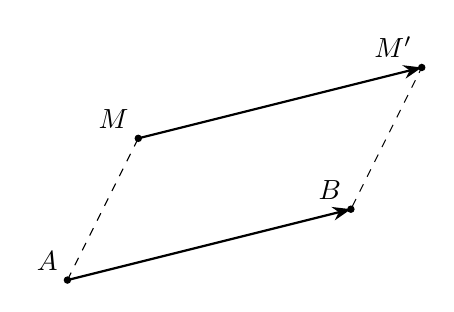
\begin{tikzpicture}[>=Stealth,scale=.9]
\coordinate(A) at (0,0);\coordinate(B) at (4,1);\coordinate(M) at (1,2);\coordinate(N) at (5,3);
\draw[dashed](A)--(M)--(N)--(B);\draw[->,thick](A)--(B);\draw[->,thick](M)--(N);
\foreach \p/\n in {A/A,B/B,M/M,N/M'}\fill(\p)circle(1.5pt) node[above left]{$\n$};
\end{tikzpicture}\end{center}
\begin{cours}[Vecteurs égaux et opposés]
$\vect{AB}=\vect{CD}$ lorsque la translation de vecteur $\vect{AB}$ transforme $C$ en $D$. Deux vecteurs non nuls sont égaux si et seulement s'ils ont même direction, même sens et même norme.
Le vecteur opposé de $\vect{AB}$ est $\vect{BA}$ : $\vect{BA}=-\vect{AB}$.
\end{cours}
\ex{Tracer un segment $[AB]$ et placer un point $C$ hors de $(AB)$. Construire $D$ tel que $\vect{AB}=\vect{CD}$. Nommer le parallélogramme obtenu. Construire $E$ tel que $\vect{CE}=-\vect{AB}$.}
\reponse[4]{$D$ se construit en reportant depuis $C$ la direction, le sens et la longueur de $\vect{AB}$. Le parallélogramme est $ABDC$, dans cet ordre. $E$ est le symétrique de $D$ par rapport à $C$, car $\vect{CE}=-\vect{CD}$.}

\fiche{Somme, différence et relation de Chasles}
\begin{cours}[Somme de vecteurs]
La somme $\vec u+\vec v$ correspond à l'enchaînement des translations de vecteurs $\vec u$ et $\vec v$. Pour tous points $A,B,C$ :
\[\boxed{\vect{AB}+\vect{BC}=\vect{AC}}\qquad\text{(relation de Chasles).}\]
On a $\vec u-\vec v=\vec u+(-\vec v)$ et $\vect{AB}+\vect{BA}=\vec0$.
\end{cours}
\begin{center}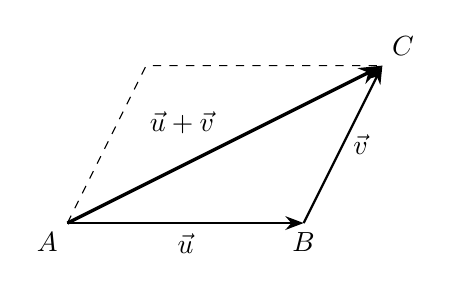
\begin{tikzpicture}[>=Stealth,scale=1.0]
\draw[->,thick](0,0)--(3,0)node[midway,below]{$\vec u$};
\draw[->,thick](3,0)--(4,2)node[midway,right]{$\vec v$};
\draw[->,very thick](0,0)--(4,2)node[midway,above left]{$\vec u+\vec v$};
\draw[dashed](0,0)--(1,2)--(4,2);
\node[below left]at(0,0){$A$};\node[below]at(3,0){$B$};\node[above right]at(4,2){$C$};
\end{tikzpicture}\end{center}
\begin{cours}[Règle du parallélogramme]
$ABDC$ est un parallélogramme si et seulement si $\vect{AD}=\vect{AB}+\vect{AC}$.
\end{cours}
\ex{Simplifier : $\vect{AB}+\vect{BC}$ ; $\vect{AB}+\vect{CA}$ ; $\vect{AB}+\vect{BC}+\vect{CD}$ ; $\vect{AB}-\vect{AC}$.}
\reponse[3.2]{$\vect{AC}$ ; $\vect{CA}+\vect{AB}=\vect{CB}$ ; $\vect{AD}$ ; $\vect{AB}+\vect{CA}=\vect{CB}$. La commutativité de l'addition permet de réordonner les vecteurs.}
\ex{Dans un parallélogramme $ABCD$, justifier que $\vect{AB}+\vect{AD}=\vect{AC}$.}
\reponse[2.4]{Dans $ABCD$, $\vect{AD}=\vect{BC}$. Donc $\vect{AB}+\vect{AD}=\vect{AB}+\vect{BC}=\vect{AC}$.}

\fiche{Produit d'un vecteur par un réel}
\begin{cours}[Définition et règles de calcul]
Pour $k\in\R$, $k\vec u=\vec0$ si $k=0$ ou $\vec u=\vec0$. Sinon, $k\vec u$ a la même direction que $\vec u$, le même sens si $k>0$, le sens opposé si $k<0$, et sa norme vaut $|k|\|\vec u\|$.
\[(k+\ell)\vec u=k\vec u+\ell\vec u,\quad k(\vec u+\vec v)=k\vec u+k\vec v,\quad k(\ell\vec u)=(k\ell)\vec u.\]
\end{cours}
\ex{Pour un vecteur $\vec u$ de norme $4$ cm, représenter $2\vec u$, $-\vec u$ et $\frac12\vec u$ à partir d'une même origine. Préciser leurs normes.}
\reponse[3.2]{Les normes sont $8$ cm, $4$ cm, $2$ cm. Les vecteurs $2\vec u$ et $\frac12\vec u$ ont le sens de $\vec u$ ; $-\vec u$ a le sens opposé.}
\begin{cours}[Caractérisations du milieu]
$I$ est le milieu de $[AB]$ si et seulement si $\vect{AI}=\vect{IB}$, ou encore $\vect{AI}=\frac12\vect{AB}$, ou $\vect{IA}+\vect{IB}=\vec0$.
\end{cours}
\ex{Dans un triangle $ABC$, $I$ est le milieu de $[AB]$ et $J$ celui de $[AC]$. Montrer que $\vect{IJ}=\frac12\vect{BC}$.}
\reponse[4.4]{Par Chasles, $\vect{IJ}=\vect{IA}+\vect{AJ}=-\frac12\vect{AB}+\frac12\vect{AC}=\frac12(\vect{BA}+\vect{AC})=\frac12\vect{BC}$. On retrouve le parallélisme des droites $(IJ)$ et $(BC)$ lorsque le triangle n'est pas aplati.}
\rituel{Réduire $3\vec u-5\vec u$ ; calculer $(-3)^2$ ; résoudre $2x+1=7$.}{$-2\vec u$ ; $9$ ; $x=3$.}

\fiche{Repères, bases et coordonnées}
\begin{cours}[Définitions]
Deux vecteurs non colinéaires $\vec i,\vec j$ forment une base du plan. Tout vecteur $\vec u$ s'écrit de manière unique $\vec u=x\vec i+y\vec j$ ; ses coordonnées sont $(x;y)$ ou $\coord{x}{y}$.
Un repère $(O;\vec i,\vec j)$ associe au point $M$ les coordonnées de $\vect{OM}$. Il est \textbf{orthonormé} si les vecteurs de base sont perpendiculaires et de norme $1$.
\end{cours}
\begin{center}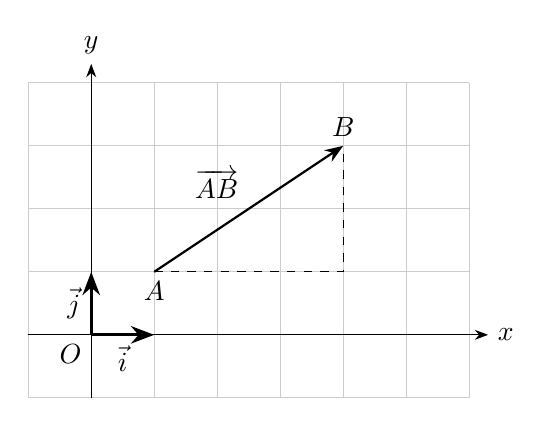
\begin{tikzpicture}[>=Stealth,scale=.8]
\draw[step=1,black!20](-1,-1)grid(6,4);\draw[->](-1,0)--(6.3,0)node[right]{$x$};\draw[->](0,-1)--(0,4.3)node[above]{$y$};
\draw[->,very thick](0,0)--(1,0)node[midway,below]{$\vec i$};\draw[->,very thick](0,0)--(0,1)node[midway,left]{$\vec j$};
\draw[->,thick](1,1)--(4,3)node[midway,above left]{$\vect{AB}$};\draw[dashed](1,1)--(4,1)--(4,3);
\node[below]at(1,1){$A$};\node[above]at(4,3){$B$};\node[below left]at(0,0){$O$};
\end{tikzpicture}\end{center}
Ici $\vect{AB}=3\vec i+2\vec j$ : on se déplace de trois unités vers la droite et deux vers le haut.
\begin{cours}[Calculs avec les coordonnées]
Si $A(x_A;y_A)$, $B(x_B;y_B)$, $\vec u(x;y)$ et $\vec v(x';y')$ :
\[\vect{AB}=\coord{x_B-x_A}{y_B-y_A},\quad \vec u+\vec v=\coord{x+x'}{y+y'},\quad k\vec u=\coord{kx}{ky}.\]
Deux vecteurs sont égaux si et seulement si leurs coordonnées respectives sont égales.
\end{cours}
\ex{Pour $\vec u(3;2)$ et $\vec v(-1;4)$, calculer $\vec u+\vec v$ et $2\vec u-\vec v$. Écrire $\vec w(5;-3)$ dans la base $(\vec i,\vec j)$.}
\reponse[2.4]{$\vec u+\vec v=(2;6)$ ; $2\vec u-\vec v=(7;0)$ ; $\vec w=5\vec i-3\vec j$.}

\fiche{Norme, distance et milieu}
\begin{cours}[Propriétés]
Dans un repère \textbf{orthonormé}, pour $\vec u(x;y)$ et deux points $A,B$ :
\[\|\vec u\|=\sqrt{x^2+y^2},\qquad AB=\sqrt{(x_B-x_A)^2+(y_B-y_A)^2}.\]
Dans tout repère, le milieu de $[AB]$ est $I\left(\frac{x_A+x_B}{2};\frac{y_A+y_B}{2}\right)$.
\end{cours}
\preuve[3]{La formule de distance découle du théorème de Pythagore appliqué aux déplacements horizontal et vertical. Pour le milieu, $\vect{AI}=\frac12\vect{AB}$ donne $x_I-x_A=\frac{x_B-x_A}{2}$ et $y_I-y_A=\frac{y_B-y_A}{2}$ ; on isole $x_I,y_I$.}
\ex{Dans un repère orthonormé, $A(3;0)$, $B(5;3)$, $C(4;0)$ et $D(6;4)$.
\begin{enumerate}
\item Calculer $\vect{AB}$, $\vect{CD}$, puis $3\vect{AB}-5\vect{CD}$.
\item Déterminer $U$ tel que $\vect{BU}=2\vect{AB}-\vect{CD}$.
\item Déterminer $E$ tel que $ABCE$ soit un parallélogramme, puis son centre $I$.
\item Calculer $AB$ et $CD$.
\end{enumerate}}
\reponse[6]{1. $\vect{AB}=(2;3)$ et $\vect{CD}=(2;4)$, donc $3\vect{AB}-5\vect{CD}=(-4;-11)$.\\
2. $\vect{BU}=(2;2)$, donc $U=B+(2;2)=(7;5)$.\\
3. $E=A+C-B=(2;-3)$. Le centre est le milieu de $[AC]$ : $I(7/2;0)$. Le milieu de $[BE]$ donne le même résultat.\\
4. $AB=\sqrt{13}$ et $CD=\sqrt{20}=2\sqrt5$.}

\fiche{Colinéarité et déterminant}
\begin{cours}[Définition]
Deux vecteurs non nuls sont colinéaires s'ils ont la même direction. Le vecteur nul est colinéaire à tout vecteur. Si $\vec v\ne\vec0$, $\vec u$ et $\vec v$ sont colinéaires si et seulement s'il existe un réel $k$ tel que $\vec u=k\vec v$.
\end{cours}
\vigilance{Dans la dernière caractérisation, la condition $\vec v\ne\vec0$ est nécessaire : un vecteur non nul ne peut pas être un multiple du vecteur nul.}
\begin{cours}[Déterminant et critère de colinéarité]
Pour $\vec u(x;y)$, $\vec v(x';y')$, $\det(\vec u,\vec v)=xy'-yx'$.
\[\vec u,\vec v\text{ colinéaires}\quad\Longleftrightarrow\quad\det(\vec u,\vec v)=0.\]
\end{cours}
\preuve[4.2]{Si $\vec u=k\vec v$, alors $xy'-yx'=kx'y'-ky'x'=0$. Le cas où un vecteur est nul est immédiat.
Réciproquement, supposons $\vec v\ne\vec0$ et $xy'-yx'=0$. Si $x'\ne0$, posons $k=x/x'$. L'égalité donne $y=ky'$, donc $\vec u=k\vec v$. Si $x'=0$, alors $y'\ne0$, d'où $x=0$ ; avec $k=y/y'$, on obtient encore $\vec u=k\vec v$.}
\ex{Étudier la colinéarité : (a) $\vec u(3;2)$ et $\vec v(-6;-5)$ ; (b) $\vec w(4;1)$ et $\vec t(3;3/4)$. Si $\vect{AB}=2\vect{CD}$ et $\vect{BD}=-5\vect{CD}$, relier $\vect{AB}$ et $\vect{BD}$.}
\reponse[3.2]{(a) $\det(\vec u,\vec v)=-15+12=-3\ne0$ : non colinéaires. (b) $\vec t=\frac34\vec w$ : colinéaires ; le déterminant vaut $4\times\frac34-3=0$. Enfin $\vect{AB}=-\frac25\vect{BD}$, y compris si les vecteurs sont nuls.}

\fiche{Alignement et parallélisme}
\begin{cours}[Applications]
Pour $A\ne B$ et $C\ne D$, les droites $(AB)$ et $(CD)$ sont parallèles (éventuellement confondues) si et seulement si $\det(\vect{AB},\vect{CD})=0$.
Les points $A,B,C$ sont alignés si et seulement si $\det(\vect{AB},\vect{AC})=0$.
\end{cours}
\ex{Montrer que $(AB)$ et $(CD)$ sont parallèles avec $A(2;-4)$, $B(10;-2)$, $C(-16;-4)$ et $D(12;3)$.}
\reponse[3.2]{$\vect{AB}=(8;2)$ et $\vect{CD}=(28;7)$. Leur déterminant vaut $8\times7-2\times28=0$. Les points de chaque paire sont distincts : les deux droites existent et sont parallèles.}
\ex{Montrer que $E(0;1/2)$, $F(2;1)$ et $G(6;2)$ sont alignés.}
\reponse[3.2]{$\vect{EF}=(2;1/2)$ et $\vect{EG}=(6;3/2)=3\vect{EF}$. Le déterminant vaut $2\times3/2-(1/2)\times6=0$ ; donc les points sont alignés.}
\ex{Avec $A(-1;1)$, $B(3;2)$, $C(-2;-3)$, $D(6;-1)$, $E(5;0)$, montrer que $(AB)\parallel(CD)$ et que $E,B,D$ sont alignés.}
\reponse[3.2]{$\vect{AB}=(4;1)$ et $\vect{CD}=(8;2)=2\vect{AB}$. Puis $\vect{EB}=(-2;2)$ et $\vect{ED}=(1;-1)=-\frac12\vect{EB}$. Les deux résultats suivent.}

\sequence{Droites du plan}{Droites du plan}{1--16 octobre 2026}
\section{Vecteur directeur et équation cartésienne}
\begin{cours}[Définition]
Un vecteur directeur d'une droite est un vecteur \textbf{non nul} ayant la direction de cette droite. Si $A\ne B$, $\vect{AB}$ dirige $(AB)$.
Toute droite admet une équation $ax+by+c=0$ avec $(a,b)\ne(0,0)$. Un vecteur directeur est $\coord{-b}{a}$.
\end{cours}
\ex{Pour $A(-2;4)$ et $B(6;2)$, calculer $\vect{AB}$ puis vérifier que $\vec u(4;-1)$ dirige $(AB)$.}
\reponse[2.4]{$\vect{AB}=(8;-2)=2\vec u$. Le vecteur $\vec u$ est non nul et colinéaire à $\vect{AB}$ ; il dirige donc $(AB)$.}
\begin{cours}[Établir une équation à l'aide du déterminant]
La droite passant par $A(x_A;y_A)$ et dirigée par $\vec u(\alpha;\beta)\ne\vec0$ a pour équation
\[\beta(x-x_A)-\alpha(y-y_A)=0.\]
\end{cours}
\preuve[4]{Un point $M(x;y)$ appartient à la droite si et seulement si $\vect{AM}$ est colinéaire à $\vec u$, y compris pour $M=A$. Or
\[\det(\vect{AM},\vec u)=(x-x_A)\beta-(y-y_A)\alpha.\]
L'annulation du déterminant donne l'équation annoncée. En développant, $a=\beta$, $b=-\alpha$ et $c=-\beta x_A+\alpha y_A$ ; comme $\vec u\ne\vec0$, $(a,b)\ne(0,0)$.}
\vigilance{Le vecteur nul ne dirige aucune droite. Le signe du déterminant dépend de l'ordre des vecteurs, mais son annulation n'en dépend pas.}

\fiche{Déterminer une équation de droite}
\begin{methode}
À partir d'un point et d'un vecteur directeur : choisir $a,b$ puis remplacer $x,y$ par les coordonnées du point pour trouver $c$. À partir de deux points distincts : calculer d'abord un vecteur directeur.
\end{methode}
\ex{Déterminer une équation cartésienne de la droite passant par $A(2;-1)$ et dirigée par $\vec u(3;2)$.}
\reponse[4]{$a=2$, $b=-3$ conviennent. La droite a donc une équation $2x-3y+c=0$. Comme $A$ lui appartient, $4+3+c=0$, d'où $c=-7$. Une équation est $2x-3y-7=0$. Vérification : $2\times2-3\times(-1)-7=0$ et $(3;2)$ est bien directeur.}
\ex{Déterminer une équation cartésienne de $(AB)$ pour $A(3;3)$ et $B(2;-2)$.}
\reponse[4]{$\vect{AB}=(-1;-5)$ dirige la droite. On peut choisir $(a,b)=(5,-1)$. Avec $A$, $15-3+c=0$, donc $c=-12$. Ainsi $5x-y-12=0$. Pour $B$, $10+2-12=0$, ce qui confirme le résultat.}
\ex{Le point $P(1;2)$ appartient-il à $d:2x-3y+4=0$ ? Le point $Q(2;1)$ lui appartient-il ?}
\reponse[2.4]{Pour $P$, $2-6+4=0$ : oui. Pour $Q$, $4-3+4=5\ne0$ : non.}

\fiche{Équation réduite, pente et fonction affine}
\begin{cours}[Définitions]
Une droite non verticale a une unique équation réduite $y=mx+p$. $m$ est la pente (coefficient directeur), $p$ l'ordonnée à l'origine. Elle représente la fonction affine $x\mapsto mx+p$ ; $(1;m)$ est un vecteur directeur.
Une droite verticale a une équation $x=k$ ; elle n'est pas la courbe d'une fonction de $x$. Une droite horizontale a une équation $y=k$.
\end{cours}
\begin{cours}[Calcul de pente]
Si $x_A\ne x_B$, la pente de $(AB)$ vaut $m=\dfrac{y_B-y_A}{x_B-x_A}$. Pour trouver $p$, on utilise ensuite $y_A=mx_A+p$.
\end{cours}
\ex{Déterminer l'équation réduite de $2x+3y-1=0$, puis tracer $d:y=-2x+3$.}
\reponse[2.4]{$3y=-2x+1$, donc $y=-\frac23x+\frac13$. Pour $d$, placer $(0;3)$ et $(1;1)$, puis tracer la droite ; un déplacement de $1$ en abscisse correspond à $-2$ en ordonnée.}
\begin{center}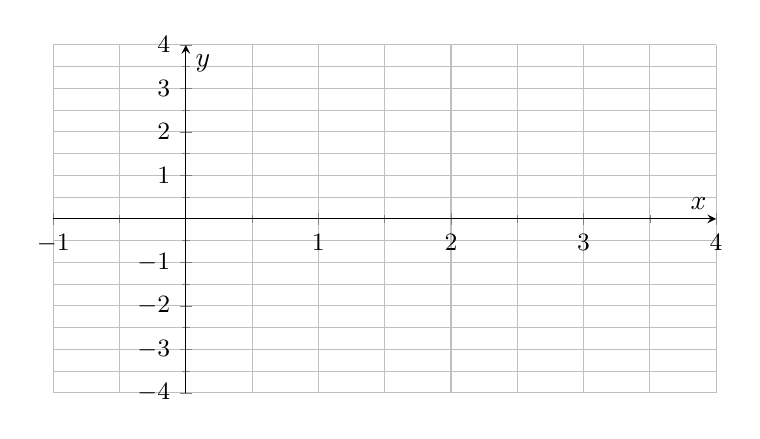
\begin{tikzpicture}\begin{axis}[coursaxe,xmin=-1,xmax=4,ymin=-4,ymax=4,width=10cm,height=6cm,xtick={-1,...,4},ytick={-4,...,4}]
\ifprof\addplot[thick,domain=-.5:3.5]{-2*x+3};\addplot[only marks]coordinates{(0,3)(1,1)};\fi
\end{axis}\end{tikzpicture}\end{center}
\ex{Trouver la fonction affine $f$ telle que $f(0)=3$ et $f(-1)=5$, puis la fonction affine $g$ dont la courbe passe par $C(-1;2)$ et $E(5;-2)$.}
\reponse[2.4]{$f(x)=-2x+3$, car $m=(3-5)/(0+1)=-2$. Pour $g$, $m=(-2-2)/(5+1)=-2/3$ et $p=2-2/3=4/3$, donc $g(x)=-\frac23x+\frac43$.}

\fiche{Positions relatives de deux droites}
\begin{cours}[Propriétés]
Deux droites sont sécantes, strictement parallèles ou confondues. Pour $y=mx+p$ et $y=m'x+p'$ :
\begin{itemize}\item si $m\ne m'$, elles sont sécantes ;\item si $m=m'$ et $p\ne p'$, elles sont strictement parallèles ;\item si $m=m'$ et $p=p'$, elles sont confondues.\end{itemize}
Pour des équations cartésiennes, on compare les directions avec le déterminant. Si les directions sont colinéaires, on teste ensuite l'appartenance d'un point pour distinguer droites confondues et strictement parallèles.
\end{cours}
\ex{Déterminer une équation de $d$ passant par $A(2;3)$ et parallèle à $d':x-3y-3=0$.}
\reponse[3.2]{$d'$ a pour vecteur directeur $(3;1)$. On cherche $d:x-3y+c=0$. Comme $A\in d$, $2-9+c=0$, donc $c=7$. Ainsi $d:x-3y+7=0$. Les deux droites sont strictement parallèles, car les constantes diffèrent pour les mêmes coefficients de $x,y$.}
\ex{Étudier les positions relatives :
\begin{enumerate}\item $2x-y+1=0$ et $4x-2y+2=0$ ;\item $x=2$ et $x=-1$ ;\item $y=2x-3$ et $y=-x+3$.\end{enumerate}}
\reponse[4]{1. La deuxième équation est le double de la première : droites confondues. 2. Deux verticales distinctes : strictement parallèles. 3. Les pentes $2$ et $-1$ diffèrent : sécantes. Leur intersection vérifie $2x-3=-x+3$, donc $x=2$ et $y=1$.}

\fiche{Intersection : résolution par substitution}
\begin{cours}[Définition]
Résoudre un système de deux équations en $x,y$, c'est trouver tous les couples $(x;y)$ vérifiant simultanément les deux équations. Pour deux équations de droites : une intersection donne un couple solution ; des droites strictement parallèles donnent aucune solution ; des droites confondues donnent une infinité de solutions.
\end{cours}
\begin{methode}[Substitution]
Isoler une inconnue dans une équation, remplacer son expression dans l'autre, résoudre puis retrouver la seconde inconnue. Vérifier le couple dans les deux équations initiales.
\end{methode}
\ex{Résoudre $\begin{cases}-2x+y+3=0,\\3x-5y-2=0.\end{cases}$}
\reponse[4]{La première équation donne $y=2x-3$. En remplaçant dans la seconde : $3x-5(2x-3)-2=0$, soit $-7x+13=0$. Ainsi $x=13/7$ puis $y=5/7$. L'ensemble solution est $S=\{(13/7;5/7)\}$. Les substitutions donnent $(-26+5+21)/7=0$ et $(39-25-14)/7=0$.}
\ex{Résoudre par substitution :
\[\text{(a) }\begin{cases}-2x+y+3=0\\x-4y+5=0\end{cases}\qquad
\text{(b) }\begin{cases}2x+3y-10=0\\4x+5y-16=0.\end{cases}\]}
\reponse[4]{(a) $y=2x-3$ puis $x-4(2x-3)+5=0$, d'où $x=17/7$, $y=13/7$.\\(b) $x=(10-3y)/2$ ; $2(10-3y)+5y-16=0$, donc $y=4$, puis $x=-1$.}

\fiche{Combinaison linéaire et Python}
\begin{methode}[Combinaison linéaire]
Multiplier les équations par des nombres non nuls pour obtenir des coefficients opposés d'une inconnue ; les additionner pour éliminer cette inconnue. Conserver une équation du système pour calculer l'autre inconnue.
\end{methode}
\ex{Résoudre $\begin{cases}2x+3y+1=0\\3x-4y-2=0.\end{cases}$ Reprendre ensuite les deux systèmes de l'exemple précédent par combinaison.}
\reponse[4.8]{Multiplier la première équation par $3$ et la seconde par $-2$ donne $6x+9y+3=0$ et $-6x+8y+4=0$. La somme donne $17y+7=0$, d'où $y=-7/17$. Puis $2x-21/17+1=0$, donc $x=2/17$.
Pour (a), ajouter quatre fois la première équation à la seconde : $-7x+17=0$, donc $(x;y)=(17/7;13/7)$. Pour (b), soustraire deux fois la première à la seconde : $-y+4=0$, donc $(x;y)=(-1;4)$.}
\begin{lstlisting}
def determinant(u, v):
    return u[0]*v[1] - u[1]*v[0]

def alignes(A, B, C):
    AB = (B[0]-A[0], B[1]-A[1])
    AC = (C[0]-A[0], C[1]-A[1])
    return determinant(AB, AC) == 0
\end{lstlisting}
\ex{Prévoir \texttt{alignes((0,0), (2,1), (6,3))} puis \texttt{alignes((0,0), (2,1), (6,4))}.}
\reponse[2]{\texttt{True}, puis \texttt{False} : les déterminants sont $0$ et $2$. Le test exact convient ici aux coordonnées entières ; les approximations flottantes demandent de tenir compte des erreurs numériques.}

\sequence{Nombres réels et intervalles}{Réels et intervalles}{2--13 novembre 2026}
\section{Les ensembles de nombres}
\begin{cours}[Définitions]
\begin{itemize}
\item $\N$ : entiers naturels ; $\Z$ : entiers relatifs.
\item $\D$ : nombres décimaux, de la forme $a/10^n$ avec $a\in\Z$, $n\in\N$.
\item $\Q$ : nombres rationnels, de la forme $a/b$ avec $a,b\in\Z$, $b\ne0$.
\item $\R$ : nombres réels, représentés par les abscisses des points d'une droite graduée. Un réel non rationnel est \textbf{irrationnel}.
\end{itemize}
\[\N\subsetneq\Z\subsetneq\D\subsetneq\Q\subsetneq\R.\]
\end{cours}
\begin{center}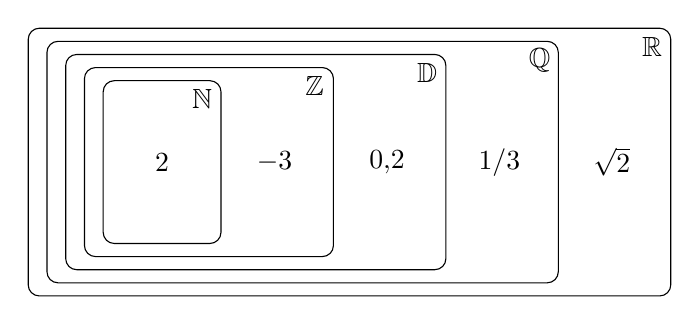
\begin{tikzpicture}[scale=.68]
\foreach \x/\w/\label in {0/12/\R,.35/9.9/\Q,.7/7.8/\D,1.05/5.7/\Z,1.4/3.6/\N}{\draw[rounded corners](\x,\x*.7)rectangle(\w,5-\x*.7);\node at(\w-.35,4.65-\x*.7){$\label$};}
\node at(2.5,2.5){$2$};\node at(4.6,2.5){$-3$};\node at(6.7,2.5){$0{,}2$};\node at(8.8,2.5){$1/3$};\node at(10.9,2.5){$\sqrt2$};
\end{tikzpicture}\end{center}
\ex{Donner le plus petit des cinq ensembles contenant chacun des nombres : $-95$ ; $7{,}29$ ; $5/3$ ; $\sqrt{25}$ ; $\sqrt2$ ; $\pi$ ; $0{,}0002$.}
\reponse[3.2]{$-95\in\Z$ ; $7{,}29\in\D$ ; $5/3\in\Q$ ; $\sqrt{25}=5\in\N$ ; $\sqrt2,\pi\in\R\setminus\Q$ ; $0{,}0002=2/10^4\in\D$. L'irrationalité de $\pi$ est admise ici.}

\fiche{Deux démonstrations par l'absurde}
\begin{methode}[Raisonnement par l'absurde]
Pour prouver une proposition, supposer sa négation, en déduire une contradiction, puis conclure que la proposition est vraie.
\end{methode}
\begin{cours}[Propriété]
$\dfrac13$ n'est pas un nombre décimal.
\end{cours}
\preuve[5]{Supposons $1/3=a/10^n$ avec $a\in\Z$, $n\in\N$. Alors $10^n=3a$ serait multiple de $3$. Pourtant $10\equiv1$ modulo $3$, donc $10^n$ a un reste de $1$ dans la division par $3$ (on peut aussi utiliser le critère de divisibilité par $3$). Contradiction. Donc $1/3\notin\D$.}
\begin{cours}[Propriété]
$\sqrt2$ est irrationnel.
\end{cours}
\preuve[6]{Supposons $\sqrt2=p/q$ avec $p,q\in\N$, $q\ne0$, et $p/q$ irréductible. Alors $p^2=2q^2$, donc $p^2$ est pair. Si $p$ était impair, son carré le serait aussi : ainsi $p$ est pair. Écrivons $p=2k$. On obtient $4k^2=2q^2$, puis $q^2=2k^2$ ; $q$ est donc pair à son tour. Ainsi $2$ divise $p$ et $q$, contrairement à l'irréductibilité. Donc $\sqrt2\notin\Q$.}
\prof{Faire identifier séparément l'hypothèse de départ, l'implication utilisée par contraposée sur la parité et la contradiction finale. Ne pas présenter une écriture décimale de calculatrice comme une preuve d'irrationalité.}

\fiche{Intervalles de la droite réelle}
\begin{cours}[Notations]
Pour deux réels $a<b$, les intervalles décrivent les réels compris entre deux bornes, avec ou sans les bornes. Un crochet fermé inclut la borne, un crochet ouvert l'exclut. Les symboles $-\infty,+\infty$ ne sont pas des réels et sont toujours accompagnés d'un crochet ouvert.
\end{cours}
\begin{center}\renewcommand{\arraystretch}{1.8}\begin{tabular}{c|c|l}
\textbf{Condition}&\textbf{Intervalle}&\textbf{Description}\\\hline
$a\leq x\leq b$&$[a;b]$&deux bornes incluses\\
$a<x\leq b$&$]a;b]$&$a$ exclu, $b$ inclus\\
$a\leq x<b$&$[a;b[$&$a$ inclus, $b$ exclu\\
$a<x<b$&$]a;b[$&deux bornes exclues\\
$x\geq a$&$[a;+\infty[$&supérieur ou égal à $a$\\
$x>a$&$]a;+\infty[$&strictement supérieur à $a$\\
$x\leq b$&$]-\infty;b]$&inférieur ou égal à $b$\\
$x<b$&$]-\infty;b[$&strictement inférieur à $b$
\end{tabular}\end{center}
\[\R=]-\infty;+\infty[,\quad \R^*=]-\infty;0[\,\cup\,]0;+\infty[.\]
\vigilance{Les réels strictement négatifs forment $]-\infty;0[$ : $0$ est exclu. $[a;a]=\{a\}$ ; $]a;a[=\varnothing$.}
\ex{Écrire sous forme d'intervalle puis représenter : $2\leq x\leq5$ ; $x>4$ ; $-6<x\leq2$ ; $x<0$.}
\reponse[4]{$[2;5]$ ; $]4;+\infty[$ ; $]-6;2]$ ; $]-\infty;0[$. Sur la droite graduée, indiquer les bornes, puis matérialiser chacune comme incluse ou exclue.}

\fiche{Intersection et réunion d'intervalles}
\begin{cours}[Définition]
$\,I\cap J$ correspond à la condition « appartenir à $I$ \textbf{et} à $J$ » ; $I\cup J$ correspond à « appartenir à $I$ \textbf{ou} à $J$ ». Une réunion d'intervalles n'est pas toujours un intervalle.
\end{cours}
\ex{Avec $I=[0;12]$ et $J=[3;20]$, déterminer $I\cap J$ et $I\cup J$.}
\reponse[2.4]{$I\cap J=[3;12]$ et $I\cup J=[0;20]$.}
\ex{Compléter, en justifiant par des représentations sur une droite graduée.}
\begin{center}\renewcommand{\arraystretch}{2}\begin{tabular}{c c|c c}
$I$&$J$&$I\cap J$&$I\cup J$\\\hline
$]-4;3]$&$[1;5]$&\trou{$[1;3]$}&\trou{$]-4;5]$}\\
$]-\infty;2]$&$[-4;+\infty[$&\trou{$[-4;2]$}&\trou{$\R$}\\
$]-\infty;7]$&$[7;+\infty[$&\trou{$\{7\}$}&\trou{$\R$}\\
$]-\infty;5]$&$[-3;+\infty[$&\trou{$[-3;5]$}&\trou{$\R$}\\
$]-2;0[$&$]0;3]$&\trou{$\varnothing$}&\trou{$]-2;0[\cup]0;3]$}
\end{tabular}\end{center}
\reponse[4]{Pour chaque intersection, conserver les points communs aux deux représentations ; pour chaque réunion, conserver tous les points de l'une au moins. Dans la dernière ligne, $0$ n'appartient à aucun intervalle : on ne peut pas remplacer la réunion par $]-2;3]$.}
\rituel{Simplifier $\vect{AB}+\vect{BC}$ ; résoudre $3x-6=0$ ; calculer $10^{-2}$.}{$\vect{AC}$ ; $x=2$ ; $0{,}01$.}

\fiche{Valeur absolue et distance}
\begin{cours}[Définition et propriétés]
$|x|$ est la distance du réel $x$ à $0$ ; $|x|\geq0$ et
\[|x|=\begin{cases}x&\text{si }x\geq0,\\-x&\text{si }x<0.\end{cases}\]
La distance entre $a$ et $b$ est $|b-a|$. Pour $a\in\R$ et $r\geq0$ :
\[|x-a|\leq r\iff x\in[a-r;a+r],\qquad |x-a|<r\iff x\in]a-r;a+r[.\]
\end{cours}
\ex{Calculer $|3{,}2|$, $|-1{,}6|$, $|\sqrt3-2|$, puis les distances entre $2$ et $5$, $2$ et $-5$, $-2$ et $-5$.}
\reponse[2.4]{$3{,}2$ ; $1{,}6$ ; $2-\sqrt3$ puisque $\sqrt3<2$. Les distances sont $3$, $7$ et $3$.}
\ex{Résoudre : $|x-7/3|=14$ ; $|x-2|\leq3$ ; $|x+3|<5$.}
\reponse[4.8]{Pour la première équation, $x-7/3=14$ ou $x-7/3=-14$, donc $S=\{-35/3;49/3\}$. Puis $|x-2|\leq3\iff x\in[-1;5]$. Enfin $|x+3|=|x-(-3)|<5\iff x\in]-8;2[$.}
\ex{Écrire $x\in[4;10]$ sous forme d'une inégalité avec valeur absolue.}
\reponse[2]{Le centre est $(4+10)/2=7$ et le rayon $(10-4)/2=3$ : $|x-7|\leq3$.}

\fiche{Encadrements et approximations}
\begin{cours}[Vocabulaire]
Encadrer $x$, c'est donner $a\leq x\leq b$ ; l'amplitude est $b-a$. Une valeur approchée par défaut est inférieure ou égale à $x$ ; une valeur approchée par excès lui est supérieure ou égale. L'arrondi choisit la valeur la plus proche à la précision demandée.
Les chiffres significatifs se comptent à partir du premier chiffre non nul ; la précision affichée doit convenir au contexte.
\end{cours}
\ex{Encadrer $\sqrt2$ par deux centièmes consécutifs. Donner son arrondi au centième. Arrondir $0{,}004567$ à trois chiffres significatifs, puis $12345$ à trois chiffres significatifs en écriture scientifique.}
\reponse[3.2]{$1{,}41^2=1{,}9881<2<2{,}0164=1{,}42^2$, donc $1{,}41<\sqrt2<1{,}42$ (amplitude $0{,}01$). L'arrondi au centième est $1{,}41$. Les autres arrondis sont $0{,}00457$ et $1{,}23\times10^4$.}
\begin{lstlisting}
def encadre_racine2(p):
    # p entier naturel ; calculs entiers exacts
    q = 10**p
    k = 0
    while (k+1)**2 <= 2*q*q:
        k = k+1
    return k/q, (k+1)/q
\end{lstlisting}
\ex{Expliquer pourquoi cette fonction encadre $\sqrt2$. Que renvoie-t-elle pour $p=2$ ? Pourquoi termine-t-elle ?}
\reponse[3.2]{La boucle cherche le plus grand entier $k$ tel que $k^2\leq2q^2$. À la sortie, $k^2\leq2q^2<(k+1)^2$, donc $k/q\leq\sqrt2<(k+1)/q$. Pour $p=2$, elle renvoie $(1{,}41;1{,}42)$. Comme $(2q)^2>2q^2$, le compteur finit par atteindre une valeur qui rend le test faux. Les divisions finales sont des approximations flottantes ; les tests de carrés sont exacts.}

\sequence{Bilan de trimestre et remédiation}{Bilan de trimestre}{16--20 novembre 2026}
\section{Bilan individuel}
\begin{methode}[Consigne]
Chercher sans le cours pendant 25 minutes, puis vérifier avec les méthodes du livret. Pour chaque question, noter : réussi seul, réussi avec aide, ou à reprendre. Justifier les réponses.
\end{methode}
\ex[Bilan des séquences 1 à 4]{\begin{enumerate}
\item Rendre $90/126$ irréductible. Démontrer que la somme de deux entiers impairs est paire.
\item Avec $A(-1;2)$ et $B(3;-2)$, calculer $\vect{AB}$, $AB$ et le milieu de $[AB]$ dans un repère orthonormé.
\item Déterminer une équation de $(AB)$ ; $C(5;-4)$ appartient-il à cette droite ?
\item Calculer $[-2;4]\cap]1;7]$ et $[-2;4]\cup]1;7]$.
\item Résoudre $|x-1|\leq4$ et expliquer pourquoi $1/3\notin\D$.
\end{enumerate}}
\reponse[9]{1. $\pgcd(90,126)=18$, donc $90/126=5/7$. Si $u=2k+1$ et $v=2\ell+1$, alors $u+v=2(k+\ell+1)$ est pair.\\2. $\vect{AB}=(4;-4)$ ; $AB=4\sqrt2$ ; milieu $I(1;0)$.\\3. $y=-x+1$. Pour $C$, $-4=-5+1$ : il appartient à $(AB)$.\\4. Intersection $]1;4]$ ; réunion $[-2;7]$.\\5. $x\in[-3;5]$. Une écriture $1/3=a/10^n$ imposerait que $10^n$ soit divisible par $3$, ce qui est impossible.}
\prof{Barème possible sur 20 : 4 points par question. Repérer séparément maîtrise du calcul, choix de méthode et qualité de la justification.}
\fiche{Corriger une erreur et reprendre une méthode}
\ex[Analyse de productions]{Corriger : (a) « $\vect{AB}=(x_A-x_B;y_A-y_B)$ » ; (b) « Le vecteur nul dirige toutes les droites » ; (c) « $|x-2|\leq3$ donne $x\in[2;3]$ » ; (d) « $1/3\approx0{,}333$, donc $1/3$ est décimal ».}
\reponse[5]{(a) Soustraire origine à extrémité : $(x_B-x_A;y_B-y_A)$. (b) Un directeur doit être non nul. (c) La distance à $2$ est au plus $3$ : $x\in[-1;5]$. (d) $0{,}333$ est différent de $1/3$ : $3\times0{,}333=0{,}999\ne1$. Une approximation décimale ne détermine pas la nature du nombre approché.}
\ex[Parcours de reprise]{\begin{enumerate}
\item Réduire $72/108$, puis $\frac34-\frac16$.
\item Avec $P(1;1)$ et $Q(5;3)$, déterminer le milieu, un directeur et une équation de $(PQ)$.
\item Déterminer $]-\infty;3]\cap[-1;+\infty[$, puis résoudre $|x+2|<1$.
\end{enumerate}}
\reponse[5]{1. $2/3$ ; $7/12$. 2. Milieu $(3;2)$, directeur $(2;1)$, équation $x-2y+1=0$. 3. Intersection $[-1;3]$ ; solution de l'inéquation $]-3;-1[$.}
\fiche{Réinvestir et s'autoévaluer}
\ex[Problème de synthèse]{Deux déplacements sont représentés par $\vec u(6;4)$ et $\vec v(9;6)$.
\begin{enumerate}\item Montrer qu'ils sont colinéaires et trouver le coefficient reliant $\vec v$ à $\vec u$.
\item Le départ est $A(-2;1)$. Déterminer les arrivées $B$ et $C$ associées aux déplacements $\vec u$ et $\vec v$.
\item Trouver une équation de la droite passant par ces trois points.
\item Un point $M(x;y)$ de cette droite doit vérifier $|x-4|\leq3$. Donner l'intervalle des abscisses possibles.
\end{enumerate}}
\reponse[7]{1. $\vec v=\frac32\vec u$. 2. $B(4;5)$ et $C(7;7)$. 3. Un directeur est $(3;2)$ ; l'équation est $2x-3y+7=0$, vérifiée par les trois points. 4. $|x-4|\leq3\iff x\in[1;7]$.}
\begin{cours}[Mon bilan]
Ma priorité : \dotfill\par L'erreur à éviter : \dotfill\par La méthode à réutiliser : \dotfill\par Un exercice à refaire sans aide : \dotfill
\end{cours}
\prof{Valider la reprise par un exercice analogue réalisé sans aide après un délai. À l'oral, demander une phrase reliant calcul et conclusion géométrique.}

\sequence{Fonctions : représentations et fonctions de référence}{Fonctions : représentations}{23 novembre--4 décembre 2026}
\section{Fonction, image et antécédent}
\begin{cours}[Définition]
Une fonction à valeurs réelles associe à chaque réel $x$ de son ensemble de définition $D_f$ un unique réel $f(x)$, appelé image de $x$. Un antécédent de $y$ est un réel $x\in D_f$ tel que $f(x)=y$. On note $f:x\mapsto f(x)$. Un nombre peut avoir aucun, un ou plusieurs antécédents.
\end{cours}
\ex{Soit $g(x)=x^2-4x+32$ sur $\R$. Calculer $g(-5)$. Soit $h(x)=3x+5$ ; déterminer l'antécédent de $6$ par $h$.}
\reponse[3.2]{$g(-5)=25+20+32=77$ : $77$ est l'image de $-5$, et $-5$ est un antécédent de $77$. Pour $h$, $3x+5=6\iff x=1/3$. L'unique antécédent est $1/3$.}
\ex{Pour la fonction carré, calculer les images de $-3$ et $3$, puis les antécédents de $9$, $0$ et $-1$.}
\reponse[3.2]{$f(-3)=f(3)=9$. Les antécédents de $9$ sont $-3,3$ ; $0$ a un seul antécédent, $0$ ; $-1$ n'en a aucun dans $\R$.}
\begin{lstlisting}
def g(x):
    return x*x - 4*x + 32
\end{lstlisting}
\ex{Distinguer \texttt{g(-5)} de \texttt{x = -5}.}
\reponse[2]{Le premier appelle la fonction et renvoie $77$. Le second affecte $-5$ à la variable \texttt{x}, sans calculer l'image par $g$.}
\fiche{Ensemble de définition}
\begin{cours}[Conditions d'existence]
$D_f$ contient les valeurs pour lesquelles le procédé définissant $f$ a un sens. Un dénominateur doit être non nul ; un nombre placé sous une racine carrée doit être positif ou nul. Respecter aussi tout domaine imposé par l'énoncé ou le contexte.
\end{cours}
\ex{Déterminer les ensembles de définition :
\[f(x)=3x^2-5x+2,\quad g(x)=\frac{2x+1}{x-4},\quad h(x)=\frac{x}{x^2-9},\quad k(x)=\sqrt{2x-6}.\]}
\reponse[5]{$D_f=\R$. $D_g=]-\infty;4[\cup]4;+\infty[$ car $x-4\ne0$. $D_h=]-\infty;-3[\cup]-3;3[\cup]3;+\infty[$ car $x^2-9\ne0$. $D_k=[3;+\infty[$ car $2x-6\geq0$.}
\vigilance{La racine carrée d'un nombre négatif n'existe pas dans $\R$ ; ce n'est pas « une racine carrée négative » que l'on exclut.}
\ex[Modéliser]{Un rectangle de périmètre $20$ m a pour largeur $x$ m. Exprimer son aire et préciser le domaine si les deux dimensions doivent être strictement positives.}
\reponse[5]{La longueur vaut $10-x$, donc $A(x)=x(10-x)$ en m$^2$. $x>0$ et $10-x>0$ donnent $D_A=]0;10[$. Si les rectangles dégénérés étaient autorisés, on pourrait prendre $[0;10]$.}
\fiche{Tableau de valeurs et courbe représentative}
\begin{cours}[Définition]
$\mathcal C_f$ est l'ensemble des points $(x;f(x))$, avec $x\in D_f$. Ainsi $M(a;b)\in\mathcal C_f\iff a\in D_f$ et $b=f(a)$.
\end{cours}
\ex{Sur $[-1;4]$, $f(x)=x^2-2x-1$. Compléter le tableau, puis tracer la courbe sur tout l'intervalle.}
\begin{center}\renewcommand{\arraystretch}{1.6}\begin{tabular}{c|rrrrrrrr}
$x$&$-1$&$-0{,}5$&$0$&$1$&$1{,}5$&$2$&$3$&$4$\\\hline
$f(x)$&\trou{$2$}&\trou{$0{,}25$}&$-1$&$-2$&\trou{$-1{,}75$}&$-1$&\trou{$2$}&\trou{$7$}
\end{tabular}\end{center}
\begin{center}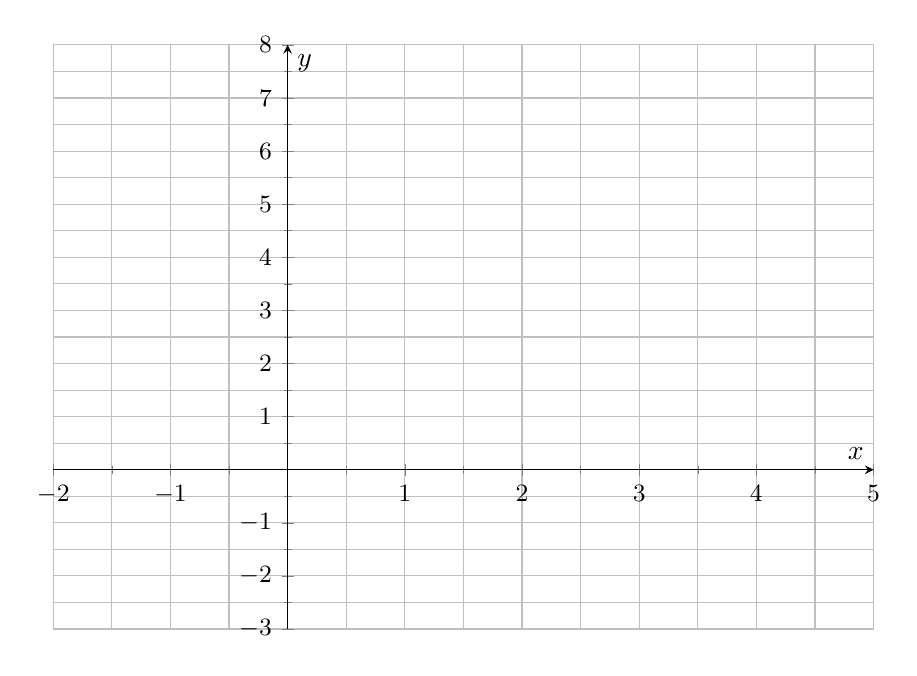
\begin{tikzpicture}\begin{axis}[coursaxe,xmin=-2,xmax=5,ymin=-3,ymax=8,width=12cm,height=9cm,xtick={-2,...,5},ytick={-3,...,8}]
\ifprof\addplot[thick,domain=-1:4]{x*x-2*x-1};\addplot[only marks]coordinates{(-1,2)(-.5,.25)(0,-1)(1,-2)(1.5,-1.75)(2,-1)(3,2)(4,7)};\fi
\end{axis}\end{tikzpicture}\end{center}
\reponse[2]{Images : $2$ ; $0{,}25$ ; $-1$ ; $-2$ ; $-1{,}75$ ; $-1$ ; $2$ ; $7$. Placer les points puis tracer la parabole. Des segments reliant ces seuls points ne donneraient qu'une approximation.}
\fiche{Résolution graphique d'équations et d'inéquations}
\begin{cours}[Méthode]
Les solutions de $f(x)=k$ sont les abscisses des intersections de $\mathcal C_f$ avec $y=k$. Pour $f(x)\leq k$, lire les abscisses où la courbe est en dessous de cette droite, intersections comprises ; avec $<$, les intersections sont exclues.
\end{cours}
\ex{La courbe représente $f(x)=1+\frac14(x+3)(x+1)(x-2)$ sur $[-4;3]$. Résoudre graphiquement $f(x)=1$, $f(x)\leq1$ et $f(x)>1$.}
\begin{center}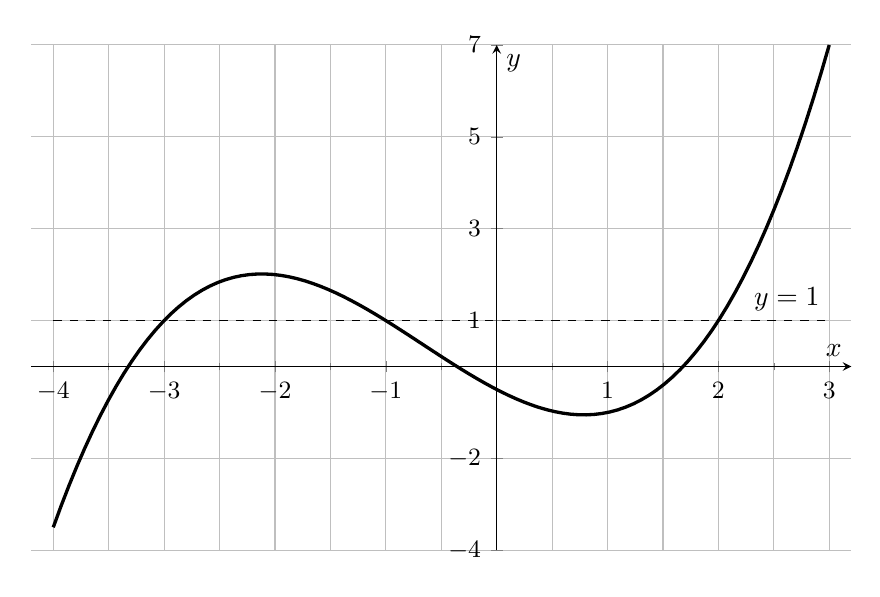
\begin{tikzpicture}\begin{axis}[coursaxe,xmin=-4.2,xmax=3.2,ymin=-4,ymax=7,xtick={-4,...,3},ytick={-4,-2,0,1,3,5,7},width=12cm,height=8cm]
\addplot[very thick,domain=-4:3]{1+(x+3)*(x+1)*(x-2)/4};\addplot[dashed,domain=-4:3]{1};\node[anchor=south east]at(axis cs:3,1){$y=1$};
\end{axis}\end{tikzpicture}\end{center}
\reponse[4]{$f(x)=1$ : $-3,-1,2$. $f(x)\leq1$ : $[-4;-3]\cup[-1;2]$. $f(x)>1$ : $]-3;-1[\cup]2;3]$. Les bornes $-4,3$ viennent du domaine. La factorisation vérifie exactement les intersections ; l'étude algébrique du signe sera consolidée en séquence 8.}
\prof{Graphique reconstruit pour remplacer une lecture ambiguë dans le livret d'origine. Distinguer conjecture graphique et validation exacte.}
\fiche{Comparer deux fonctions ; lire un signe}
\begin{cours}[Méthode]
$f(x)=g(x)$ se lit aux intersections des courbes. Pour $f(x)<g(x)$, $\mathcal C_f$ est strictement en dessous de $\mathcal C_g$ à la même abscisse. Le signe de $f(x)$ se lit par rapport à l'axe des abscisses.
\end{cours}
\ex{Sur $[-3;3]$, $f(x)=x^2$ et $g(x)=x+2$. Résoudre $f=g$, $f<g$, $f\geq g$ et déterminer le signe de $g$.}
\begin{center}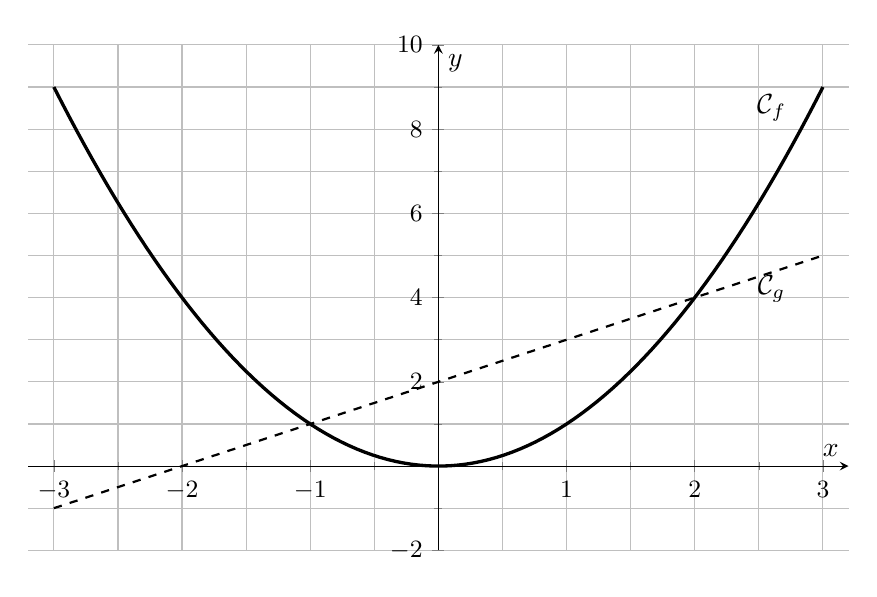
\begin{tikzpicture}\begin{axis}[coursaxe,xmin=-3.2,xmax=3.2,ymin=-2,ymax=10,width=12cm,height=8cm,xtick={-3,...,3},ytick={-2,0,2,4,6,8,10}]
\addplot[very thick,domain=-3:3]{x*x};\addplot[thick,dashed,domain=-3:3]{x+2};\node at(axis cs:2.6,8.5){$\mathcal C_f$};\node at(axis cs:2.6,4.2){$\mathcal C_g$};
\end{axis}\end{tikzpicture}\end{center}
\reponse[4]{$f=g$ pour $x=-1,2$ ; $f<g$ sur $]-1;2[$ ; $f\geq g$ sur $[-3;-1]\cup[2;3]$. $g$ est strictement négative sur $[-3;-2[$, nulle en $-2$, strictement positive sur $]-2;3]$. Signe et variations sont des informations différentes.}
\fiche{Fonctions affines et valeur absolue}
\begin{cours}[Définitions]
Une fonction affine est $f(x)=mx+p$ sur $\R$. Elle est linéaire si $p=0$, constante si $m=0$. Pour $m\ne0$, elle s'annule en $-p/m$ ; son signe est celui de $m$ à droite de ce nombre.
La fonction $x\mapsto|x|$ est définie sur $\R$, positive ou nulle, et s'annule uniquement en $0$.
\end{cours}
\ex{Classer (plusieurs réponses possibles) en affine, linéaire, constante : $5x+2$ ; $5x$ ; $7+2x-7$ ; $6$ ; $6(4x-2)$ ; $6x+5-6x$.}
\reponse[2.4]{Toutes sont affines. $5x$ et $2x$ sont linéaires ; $6$ et $5$ sont constantes ; $24x-12$ n'est ni linéaire ni constante.}
\begin{center}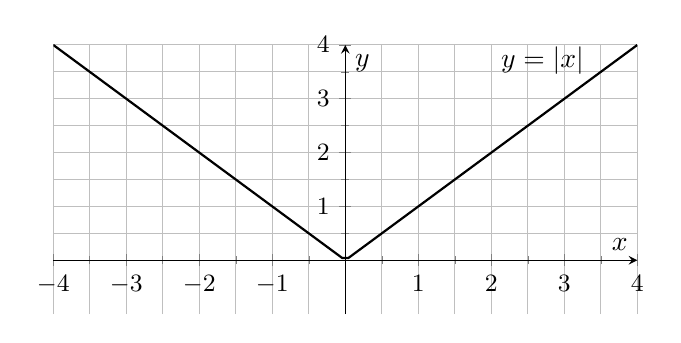
\begin{tikzpicture}\begin{axis}[coursaxe,xmin=-4,xmax=4,ymin=-1,ymax=4,width=9cm,height=5cm,xtick={-4,...,4},ytick={0,...,4}]
\addplot[thick,domain=-4:4]{abs(x)};\node at(axis cs:2.7,3.7){$y=|x|$};\end{axis}\end{tikzpicture}\end{center}
\begin{cours}[Équations et inéquations]
Si $k<0$, $|x|=k$ et $|x|\leq k$ n'ont aucune solution, et $|x|\geq k$ est vraie sur $\R$. Si $k=0$, les deux premières donnent $x=0$, la troisième est vraie sur $\R$. Pour $k>0$ :
\[|x|=k\iff x\in\{-k;k\},\quad |x|\leq k\iff x\in[-k;k],\]
\[|x|\geq k\iff x\in]-\infty;-k]\cup[k;+\infty[.\]
\end{cours}
\ex{Résoudre $|x|=5$, $|x|=-3$, $|x|\leq3$, $|x|\geq4$.}
\reponse[1.6]{$\{-5;5\}$ ; $\varnothing$ ; $[-3;3]$ ; $]-\infty;-4]\cup[4;+\infty[$.}
\fiche{Fonctions carré et inverse}
\begin{cours}[Définitions et signe]
$x\mapsto x^2$ est définie sur $\R$ ; sa courbe est une parabole. $x^2\geq0$, avec égalité seulement en $0$.
$x\mapsto1/x$ est définie sur $\R^*$ ; sa courbe est une hyperbole. $1/x$ a le signe de $x$ et ne s'annule jamais.
\end{cours}
\begin{center}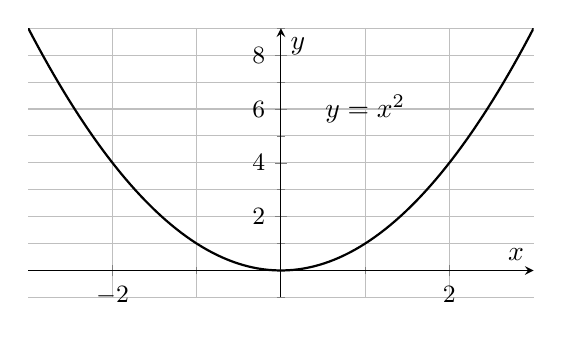
\begin{tikzpicture}\begin{axis}[coursaxe,xmin=-3,xmax=3,ymin=-1,ymax=9,width=8cm,height=5cm,xtick={-2,0,2}]
\addplot[thick,domain=-3:3]{x*x};\node at(axis cs:1,6){$y=x^2$};\end{axis}\end{tikzpicture}
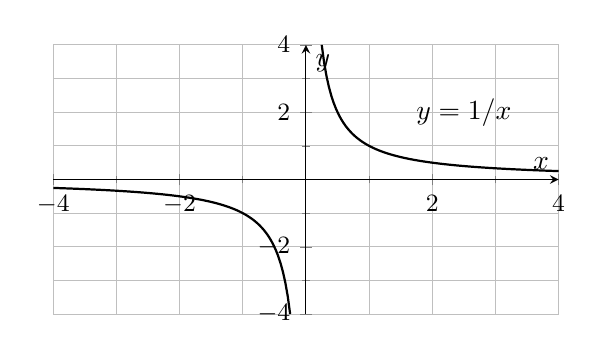
\begin{tikzpicture}\begin{axis}[coursaxe,xmin=-4,xmax=4,ymin=-4,ymax=4,width=8cm,height=5cm,xtick={-4,-2,0,2,4}]
\addplot[thick,domain=-4:-.25]{1/x};\addplot[thick,domain=.25:4]{1/x};\node at(axis cs:2.5,2){$y=1/x$};\end{axis}\end{tikzpicture}\end{center}
\begin{cours}[Équations et inéquations avec $x^2$]
Si $k<0$, $x^2=k$ et $x^2\leq k$ n'ont pas de solution ; $x^2\geq k$ est vraie sur $\R$. Si $k=0$, les deux premières donnent $x=0$, la troisième est vraie sur $\R$. Pour $k>0$ :
\[x^2=k\iff x\in\{-\sqrt k;\sqrt k\},\quad x^2\leq k\iff x\in[-\sqrt k;\sqrt k],\]
\[x^2\geq k\iff x\in]-\infty;-\sqrt k]\cup[\sqrt k;+\infty[.\]
\end{cours}
\ex{Résoudre $x^2=4$, $x^2=-1$, $x^2\geq4$, $x^2\geq-1$, $1/x=4$, $1/x=0$.}
\reponse[3.2]{$\{-2;2\}$ ; $\varnothing$ ; $]-\infty;-2]\cup[2;+\infty[$ ; $\R$ ; $\{1/4\}$ ; $\varnothing$. Plus généralement, $1/x=k$ a l'unique solution $1/k$ si $k\ne0$, aucune si $k=0$.}
\fiche{Inéquations avec la fonction inverse}
\begin{methode}
Respecter $x\ne0$ et lire les deux branches de l'hyperbole. Ne pas multiplier une inéquation par $x$ sans connaître son signe.
\end{methode}
\begin{center}\small\renewcommand{\arraystretch}{2.5}\begin{tabular}{c|c|c|c}
&$k<0$&$k=0$&$k>0$\\\hline
$1/x\leq k$&$[1/k;0[$&$]-\infty;0[$&$]-\infty;0[\cup[1/k;+\infty[$\\
$1/x\geq k$&$]-\infty;1/k]\cup]0;+\infty[$&$]0;+\infty[$&$]0;1/k]$
\end{tabular}\end{center}
\ex{Résoudre $1/x\geq2$, $1/x\leq-1$, $1/x<1/2$ et $1/x>-2$.}
\reponse[5]{$]0;1/2]$ ; $[-1;0[$ ; $]-\infty;0[\cup]2;+\infty[$ ; $]-\infty;-1/2[\cup]0;+\infty[$. Une inégalité stricte exclut l'intersection avec $y=k$ ; $0$ est toujours interdit.}
\ex{Un élève écrit : « $1/x\leq2\iff1\leq2x$, donc $x\geq1/2$ ». Que manque-t-il ?}
\reponse[4]{Il a supposé implicitement $x>0$. Pour $x<0$, $1/x<0<2$ : ces valeurs conviennent aussi. L'ensemble correct est $]-\infty;0[\cup[1/2;+\infty[$. Le nombre $-1$ réfute son équivalence.}
\fiche{Mobiliser racine carrée et cube}
\begin{cours}[Définitions]
$x\mapsto\sqrt x$ est définie sur $[0;+\infty[$ et à valeurs positives ou nulles. Pour $k\geq0$, $\sqrt x=k\iff x=k^2$ ; pour $k<0$, aucune solution.
$x\mapsto x^3$ est définie sur $\R$. Chaque réel $k$ possède un unique antécédent, noté $\sqrt[3]{k}$.
\end{cours}
\begin{center}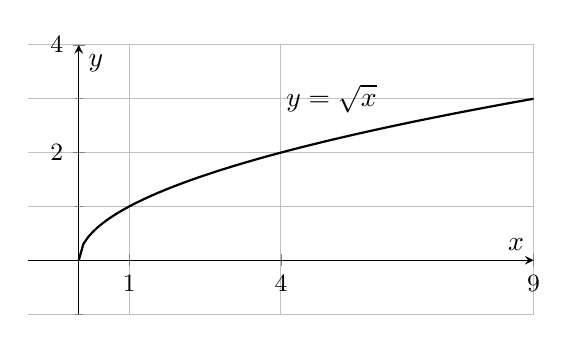
\begin{tikzpicture}\begin{axis}[coursaxe,xmin=-1,xmax=9,ymin=-1,ymax=4,width=8cm,height=5cm,xtick={0,1,4,9}]
\addplot[thick,domain=0:9]{sqrt(x)};\node at(axis cs:5,3){$y=\sqrt x$};\end{axis}\end{tikzpicture}
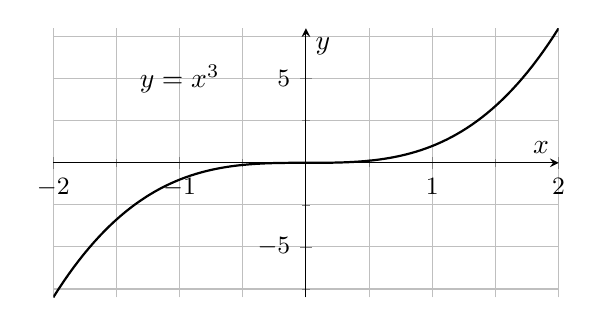
\begin{tikzpicture}\begin{axis}[coursaxe,xmin=-2,xmax=2,ymin=-8,ymax=8,width=8cm,height=5cm,xtick={-2,-1,0,1,2}]
\addplot[thick,domain=-2:2]{x*x*x};\node at(axis cs:-1,5){$y=x^3$};\end{axis}\end{tikzpicture}\end{center}
\ex{Résoudre $\sqrt x=3$ ; $\sqrt x=-2$ ; $\sqrt x\leq2$ ; $\sqrt x>3$ ; $x^3=-8$ ; $x^3\leq27$.}
\reponse[4]{$\{9\}$ ; $\varnothing$ ; $[0;4]$ ; $]9;+\infty[$ ; $\{-2\}$ ; $]-\infty;3]$. Respecter le domaine pour les racines carrées. La fonction cube conserve l'ordre.}
\ex{Comparer $x^2$ et $x$ pour $x=1/2$, puis $x=2$. Le carré d'un positif est-il toujours plus grand que lui ?}
\reponse[2.4]{$1/4<1/2$ mais $4>2$. L'affirmation est fausse ; $1/2$ est un contre-exemple. Étude générale en séquence 10.}

\sequence{Statistiques descriptives à une variable}{Statistiques descriptives}{7--18 décembre 2026}
\section{Effectifs, fréquences et moyenne}
\begin{cours}[Définitions]
Une série décrit un caractère sur une population. Si la valeur $x_i$ apparaît $n_i$ fois, $n_i$ est son effectif. L'effectif total non nul est $N=\sum_{i=1}^{p}n_i$ ; sa fréquence est $f_i=n_i/N$. La moyenne est
\[\overline x=\frac{\sum_{i=1}^{p}n_ix_i}{N}=\sum_{i=1}^{p}f_ix_i.\]
L'étendue est $x_{\max}-x_{\min}$.
\end{cours}
\ex[Pointures -- données du livret]{On étudie les pointures de $30$ élèves :
\begin{center}\small\begin{tabular}{rrrrrrrrrrrrrrr}
36&42&40&41&41&38&39&43&42&42&42&40&36&40&39\\
41&40&38&44&42&40&42&43&38&43&36&41&41&44&43
\end{tabular}\end{center}
Compléter les effectifs, calculer les fréquences, la moyenne et l'étendue.}
\begin{center}\renewcommand{\arraystretch}{1.6}\begin{tabular}{c|rrrrrrrrr}
Pointure&36&37&38&39&40&41&42&43&44\\\hline
Effectif&\trou{3}&\trou{0}&\trou{3}&\trou{2}&\trou{5}&\trou{5}&\trou{6}&\trou{4}&\trou{2}
\end{tabular}\end{center}
\reponse[6]{Effectifs : $3,0,3,2,5,5,6,4,2$, de somme $30$. Les fréquences sont ces effectifs divisés par $30$, soit en pourcentage $10$ ; $0$ ; $10$ ; environ $6{,}67$ ; $16{,}67$ ; $16{,}67$ ; $20$ ; $13{,}33$ ; $6{,}67$.
$\sum n_ix_i=1217$, donc $\overline x=1217/30\approx40{,}57$. L'étendue vaut $8$. La moyenne n'est pas forcément une valeur de la série. La somme des pourcentages arrondis peut différer légèrement de $100$.}
\fiche{Médiane et effectifs cumulés}
\begin{cours}[Définition et convention]
Une médiane est un nombre tel qu'au moins la moitié des valeurs lui soient inférieures ou égales, et au moins la moitié supérieures ou égales.
Dans la série ordonnée de $N$ valeurs, si $N$ est impair, prendre le rang $(N+1)/2$ ; si $N$ est pair, choisir la moyenne des valeurs de rangs $N/2$ et $N/2+1$.
\end{cours}
\vigilance{Avec des répétitions, plus de $50\,\%$ des valeurs peuvent être inférieures ou égales à la médiane.}
\ex{Compléter les effectifs cumulés croissants (ECC) des pointures et déterminer la médiane.}
\begin{center}\renewcommand{\arraystretch}{1.7}\begin{tabular}{c|rrrrrrrrr}
Pointure&36&37&38&39&40&41&42&43&44\\\hline
Effectif&3&0&3&2&5&5&6&4&2\\
ECC&\trou{3}&\trou{3}&\trou{6}&\trou{8}&\trou{13}&\trou{18}&\trou{24}&\trou{28}&\trou{30}
\end{tabular}\end{center}
\reponse[4]{Les rangs centraux sont $15$ et $16$. Les ECC passent de $13$ pour $40$ à $18$ pour $41$ : les deux valeurs centrales valent $41$, donc $M_e=41$. Au moins la moitié des pointures sont inférieures ou égales à $41$, et au moins la moitié supérieures ou égales à $41$.}
\ex{Calculer les médianes de $1;2;2;8;9$ et de $1;2;8;9$.}
\reponse[3.2]{La troisième valeur de la première série vaut $2$. Dans la seconde, $(2+8)/2=5$ ; la médiane choisie n'est pas une valeur de la série.}
\fiche{Quartiles et diagramme en boîte}
\begin{cours}[Définitions]
Le premier quartile $Q_1$ est la valeur de rang $\lceil N/4\rceil$ : la plus petite valeur de la série telle qu'au moins $25\,\%$ des valeurs lui soient inférieures ou égales. $Q_3$ est la valeur de rang $\lceil3N/4\rceil$.
L'écart interquartile est $Q_3-Q_1$. Le diagramme en boîte indique minimum, $Q_1$, médiane, $Q_3$, maximum.
\end{cours}
\ex{Déterminer $Q_1$, $Q_3$ et l'écart interquartile des pointures, puis tracer le diagramme en boîte.}
\reponse[3.2]{$N/4=7{,}5$ : rang $8$, donc $Q_1=39$. $3N/4=22{,}5$ : rang $23$, donc $Q_3=42$. Écart interquartile $3$. Le diagramme utilise $(36;39;41;42;44)$.}
\begin{center}\begin{tikzpicture}[x=1.5cm,y=1cm]
\draw[->](-.5,0)--(8.5,0);\foreach \x in {36,...,44}{\draw(\x-36,-.1)--(\x-36,.1)node[below=3pt]{$\x$};}
\ifprof\draw[thick](0,1)--(3,1)(6,1)--(8,1);\draw[thick](3,.5)rectangle(6,1.5);\draw[thick](5,.5)--(5,1.5)(0,.7)--(0,1.3)(8,.7)--(8,1.3);\else\path(0,1.8);\fi
\end{tikzpicture}\end{center}
\ex{Déterminer les quartiles de $1;2;2;3;4;4;4;5$. Y a-t-il exactement $25\,\%$ des valeurs inférieures ou égales à $Q_1$ ?}
\reponse[4]{$Q_1=2$ (rang $2$), $Q_3=4$ (rang $6$). Ici $3/8=37{,}5\,\%$ des valeurs sont inférieures ou égales à $Q_1$. Il faut dire « au moins ».}
\fiche{Ajout ou suppression d'une valeur}
\begin{cours}[Propriétés]
Ajouter $a$ à une série de taille $N$ donne $\overline x'=(N\overline x+a)/(N+1)$.
Retirer une occurrence de $a$, pour $N>1$, donne $\overline x'=(N\overline x-a)/(N-1)$. Utiliser la somme exacte, sans arrondi intermédiaire. Réexaminer la médiane dans la nouvelle série ordonnée.
\end{cours}
\ex{Dans la série des pointures, la somme vaut $1217$, la médiane $41$.
\begin{enumerate}\item Ajouter une pointure $36$ et calculer les nouveaux indicateurs.\item Repartir de la série initiale, retirer une pointure $44$ et recommencer.\end{enumerate}}
\reponse[5]{1. Somme $1253$, effectif $31$ : $\overline x'=1253/31\approx40{,}42$. Le rang central $16$ donne toujours $41$. 2. Somme $1173$, effectif $29$ : $\overline x''=1173/29\approx40{,}45$. Le rang central $15$ donne $41$. La moyenne diminue dans les deux cas ; la médiane reste inchangée. Les situations sont indépendantes.}
\ex{Justifier qu'ajouter la moyenne ne change pas la moyenne. L'étendue peut-elle diminuer lors d'un ajout ?}
\reponse[4]{Si $a=\overline x$, $(N\overline x+\overline x)/(N+1)=\overline x$. Lors d'un ajout, le minimum ne peut qu'être conservé ou diminuer, le maximum être conservé ou augmenter : l'étendue ne diminue pas. Lors d'une suppression, elle n'augmente pas.}
\fiche{Variance et écart type}
\begin{cours}[Définitions]
$V=\dfrac{\sum n_i(x_i-\overline x)^2}{N}$ est la variance ; $\sigma=\sqrt V$ est l'écart type. Il mesure la dispersion autour de la moyenne et a la même unité que les données. On peut aussi calculer $V=\dfrac{\sum n_ix_i^2}{N}-\overline x^{\,2}$.
\end{cours}
\ex{Calculer la variance et l'écart type des pointures.}
\reponse[4]{$\sum n_ix_i^2=49519$, donc
\[V=\frac{49519}{30}-\left(\frac{1217}{30}\right)^2=\frac{4481}{900}\approx4{,}979.\]
$\sigma=\sqrt{4481}/30\approx2{,}23$. L'écart type n'est pas la distance maximale à la moyenne.}
\ex{Comparer $A:8;10;12$ et $B:0;10;20$ avec les couples moyenne--écart type et médiane--écart interquartile.}
\reponse[5]{Les moyennes et médianes valent toutes $10$. $V_A=8/3$, $\sigma_A\approx1{,}63$ ; $V_B=200/3$, $\sigma_B\approx8{,}16$. Quartiles : $8,12$ pour $A$ ; $0,20$ pour $B$. Écarts interquartiles $4$ et $20$. $B$ est beaucoup plus dispersée malgré des centres identiques.}
\prof{La variance descriptive divise par $N$, sans correction par $N-1$. Vérifier aussi la convention de quartiles des logiciels.}
\fiche{Linéarité de la moyenne}
\begin{cours}[Propriété]
Remplacer chaque $x_i$ par $kx_i+c$ donne une moyenne $k\overline x+c$, un écart type $|k|\sigma$ et une variance $k^2V$. Ajouter une constante ne change ni variance ni écart type.
\end{cours}
\ex{Moyenne initiale $12/20$, écart type $3$. Calculer les nouveaux indicateurs pour trois modifications indépendantes, sans plafonnement des notes : ajouter $1{,}5$ ; multiplier par $0{,}8$ ; multiplier par $1{,}1$ puis ajouter $0{,}5$.}
\reponse[4]{Moyennes : $13{,}5$, $9{,}6$, $13{,}7$. Écarts types : $3$, $2{,}4$, $3{,}3$. Multiplier les notes par $1{,}1$ les augmente ; cela ne signifie pas augmenter la difficulté de l'évaluation. Avec un plafonnement à $20$, la transformation ne serait plus affine sur toutes les données.}
\begin{lstlisting}
from math import sqrt

def moyenne_ecart_type(valeurs):
    n = len(valeurs)
    if n == 0:
        raise ValueError("liste vide")
    m = sum(valeurs)/n
    v = sum((x-m)**2 for x in valeurs)/n
    return m, sqrt(v)
\end{lstlisting}
\ex{Expliquer le programme ; prévoir son résultat pour \texttt{[8, 10, 12]}.}
\reponse[3.2]{Il vérifie que la liste est non vide, calcule la moyenne, la moyenne des carrés des écarts, puis sa racine. Résultat : $(10;\sqrt{8/3})\approx(10;1{,}633)$.}
\fiche{Séries continues regroupées en classes}
\begin{cours}[Définitions et perte d'information]
Une variable quantitative continue peut prendre toutes les valeurs d'un intervalle. Ici, les observations sont regroupées en classes de même amplitude ; le centre de $[a;b[$ vaut $(a+b)/2$.
Si les moyennes $m_i$ des classes sont connues, la moyenne globale exacte est $\sum n_im_i/N$. À défaut, les remplacer par les centres donne une estimation justifiée par un modèle uniforme dans chaque classe.
\end{cours}
\ex[Tailles -- données du livret]{Compléter, estimer la moyenne à partir des centres et déterminer la classe médiane.}
\begin{center}\renewcommand{\arraystretch}{1.7}\begin{tabular}{c|ccccc}
Classe (cm)&$[150;160[$&$[160;170[$&$[170;180[$&$[180;190[$&$[190;200[$\\\hline
Effectif&8&22&35&28&7\\
Fréquence (\%)&\trou{8}&\trou{22}&\trou{35}&\trou{28}&\trou{7}\\
Centre (cm)&\trou{155}&\trou{165}&\trou{175}&\trou{185}&\trou{195}\\
ECC&\trou{8}&\trou{30}&\trou{65}&\trou{93}&\trou{100}
\end{tabular}\end{center}
\reponse[4]{Amplitude $10$ cm, effectif total $100$. Fréquences en pourcentage : $8,22,35,28,7$. Centres : $155,165,175,185,195$ cm. La somme pondérée des centres vaut $17540$, donc la moyenne estimée est $175{,}4$ cm. Les rangs centraux $50,51$ se trouvent dans $[170;180[$, classe médiane.}
\ex{Si les moyennes exactes des classes étaient $154;166;174;184;196$ cm, quelle serait la moyenne globale ?}
\reponse[2.4]{$(8\times154+22\times166+35\times174+28\times184+7\times196)/100=174{,}98$ cm.}
\fiche{Histogramme et fréquences cumulées}
\begin{cours}[Représentations]
L'aire de chaque rectangle d'un histogramme est proportionnelle à l'effectif. À amplitudes égales, les hauteurs peuvent être les effectifs. Le polygone des fréquences cumulées joint les points (borne supérieure ; fréquence cumulée), en commençant à la première borne inférieure avec $0$.
\end{cours}
\ex{Construire les deux graphiques pour les tailles de l'exemple précédent.}
\begin{center}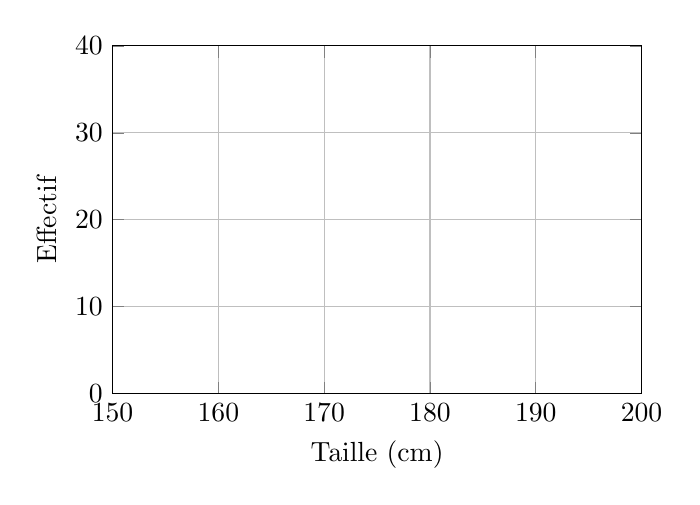
\begin{tikzpicture}\begin{axis}[width=8.3cm,height=6cm,xmin=150,xmax=200,ymin=0,ymax=40,xlabel={Taille (cm)},ylabel={Effectif},xtick={150,160,...,200},ytick={0,10,20,30,40},grid=major]
\ifprof\addplot[ybar interval,fill=black!15,draw=black]coordinates{(150,8)(160,22)(170,35)(180,28)(190,7)(200,0)};\fi
\end{axis}\end{tikzpicture}
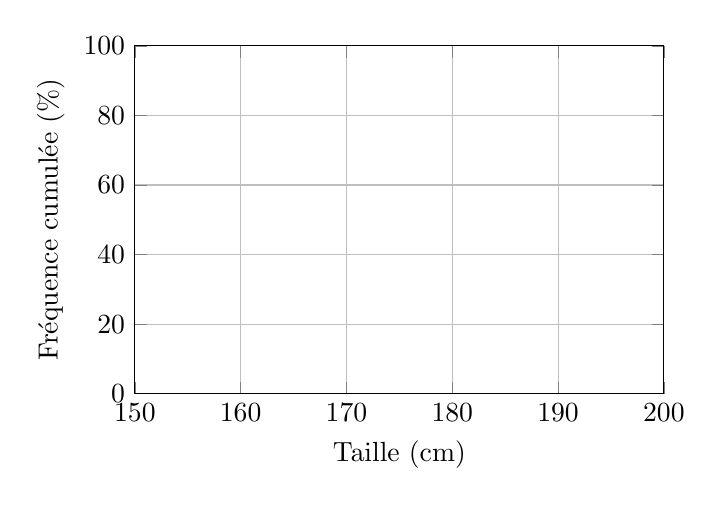
\begin{tikzpicture}\begin{axis}[width=8.3cm,height=6cm,xmin=150,xmax=200,ymin=0,ymax=100,xlabel={Taille (cm)},ylabel={Fréquence cumulée (\%)},xtick={150,160,...,200},ytick={0,20,...,100},grid=major]
\ifprof\addplot[thick,mark=*]coordinates{(150,0)(160,8)(170,30)(180,65)(190,93)(200,100)};\fi
\end{axis}\end{tikzpicture}\end{center}
\begin{methode}[Estimer la médiane]
Sous l'hypothèse d'uniformité dans $[170;180[$, la fréquence cumulée passe linéairement de $30\,\%$ à $65\,\%$. Rechercher l'abscisse correspondant à $50\,\%$.
\end{methode}
\ex{Calculer cette estimation et préciser sa portée.}
\reponse[4]{On résout $(m-170)/10=(50-30)/(65-30)$, d'où $m=170+10\times20/35\approx175{,}71$ cm. Il s'agit d'une estimation sous hypothèse d'uniformité, pas de la médiane exacte des données individuelles. Les effectifs des classes seuls ne déterminent pas cette dernière.}

\sequence{Calcul algébrique, équations et inéquations}{Calcul algébrique}{4--20 janvier 2027}
\section{Parenthèses et distributivité}
\begin{methode}[Supprimer des parenthèses]
Après un signe $+$, supprimer les parenthèses conserve les signes des termes. Après un signe $-$, chaque terme à l'intérieur change de signe. Cette règle concerne une somme ou une différence de termes.
\end{methode}
\ex{Supprimer les parenthèses et réduire : $A=x+(2+3x)$ ; $B=x-(2+3x)$ ; $C=-2x+(-4+5x)$ ; $D=-2x-(-4+5x)$.}
\reponse[3.2]{$A=4x+2$ ; $B=-2x-2$ ; $C=3x-4$ ; $D=-7x+4$.}
\begin{cours}[Distributivité]
Pour tous réels $a,b,c,d$ :
\[b(c+d)=bc+bd,\qquad(a+b)(c+d)=ac+ad+bc+bd.\]
\end{cours}
\ex{Développer et réduire :
\begin{align*}
A&=-4(8x+7)+(-8x+5)(5x+9),\\
B&=(6x+9)(-x+7)+(3x+5)(-9x+6),\\
C&=-9(-x-7)-(-x+3)(-8x-8),\\
D&=-5(-6x-7)+(x-7)(5x+8).
\end{align*}}
\reponse[5]{On développe chaque produit, puis on regroupe les termes de même degré :
\begin{align*}
A&=-32x-28-40x^2-72x+25x+45=-40x^2-79x+17,\\
B&=-6x^2+33x+63-27x^2-27x+30=-33x^2+6x+93,\\
C&=9x+63-(8x^2-16x-24)=-8x^2+25x+87,\\
D&=30x+35+5x^2-27x-56=5x^2+3x-21.
\end{align*}}

\fiche{Factoriser avec un facteur commun}
\begin{cours}[Propriété]
$ka+kb=k(a+b)$ et $ka-kb=k(a-b)$. Factoriser transforme une somme en un produit ; développer fait l'opération inverse.
\end{cours}
\ex{Factoriser :
\begin{align*}
A&=15x^2-21x,\\B&=3(2+3x)-(5+2x)(2+3x),\\
C&=(4x-1)(x+6)+(4x-1),\\D&=(1-6x)^2-(1-6x)(2+5x).
\end{align*}}
\reponse[6]{
$A=3x(5x-7)$.\\
$B=(2+3x)[3-(5+2x)]=(2+3x)(-2-2x)=-2(2+3x)(1+x)$.\\
$C=(4x-1)[(x+6)+1]=(4x-1)(x+7)$.\\
$D=(1-6x)[(1-6x)-(2+5x)]=(1-6x)(-1-11x)=(6x-1)(11x+1)$.
Vérifier les facteurs en redéveloppant.}
\ex{Choisir une forme utile de $f(x)=(x-2)(x+3)$ pour calculer $f(2)$, $f(0)$ et chercher ses zéros.}
\reponse[3.2]{La forme factorisée donne immédiatement $f(2)=0$ et les zéros $2,-3$. En $0$, $f(0)=(-2)\times3=-6$ ; la forme développée $x^2+x-6$ donne aussi ce résultat. Le choix dépend de la question.}

\fiche{Identités remarquables : développer}
\begin{cours}[Identités]
\[(a+b)^2=a^2+2ab+b^2,\qquad(a-b)^2=a^2-2ab+b^2,\]
\[(a+b)(a-b)=a^2-b^2.\]
\end{cours}
\preuve[3.2]{Développer $(a+b)(a+b)$ : $a^2+ab+ba+b^2=a^2+2ab+b^2$. Remplacer $b$ par $-b$ donne la deuxième identité. Enfin $(a+b)(a-b)=a^2-ab+ab-b^2=a^2-b^2$.}
\ex{Développer $(x+3)^2$, $(3x-4)^2$, $(x-3)(x+3)$, $(2x+3)(2x-3)$, $(4-3x)(3x+4)$.}
\reponse[3.2]{$x^2+6x+9$ ; $9x^2-24x+16$ ; $x^2-9$ ; $4x^2-9$ ; $16-9x^2$. Dans le dernier produit, réordonner $3x+4$ en $4+3x$.}
\ex{Développer et réduire $A=(2x-3)^2+(x+5)(3-x)$ et $B=2(x+3)+(2x+3)(2x-3)$.}
\reponse[4]{$A=4x^2-12x+9-x^2-2x+15=3x^2-14x+24$. $B=2x+6+4x^2-9=4x^2+2x-3$.}

\fiche{Identités remarquables : factoriser}
\begin{methode}
Repérer les deux carrés ; pour les formes à trois termes, vérifier le double produit $2ab$. Pour une différence de deux carrés, utiliser $a^2-b^2=(a-b)(a+b)$.
\end{methode}
\ex{Factoriser :
\[A=x^2-2x+1,\quad B=25+16x^2-40x,\quad C=4x^2+12x+9,\]
\[D=1-49x^2,\quad E=9x^2-4,\quad F=(2x+3)^2-64.\]}
\reponse[6]{
$A=(x-1)^2$. $B=(4x-5)^2$. $C=(2x+3)^2$.\\
$D=(1-7x)(1+7x)$. $E=(3x-2)(3x+2)$.\\
$F=[(2x+3)-8][(2x+3)+8]=(2x-5)(2x+11)$.
Pour les trois premiers, vérifier le terme intermédiaire ; pour $F$, traiter $2x+3$ comme un seul bloc.}
\ex[Contrôler une identité]{Les égalités $(a+b)^2=a^2+b^2$ et $a^2+b^2=(a-b)(a+b)$ sont-elles vraies pour tous réels ?}
\reponse[3.2]{Non : pour $a=b=1$, la première donnerait $4=2$ et la seconde $2=0$. Le terme manquant dans la première est $2ab$ ; le produit de la seconde vaut $a^2-b^2$.}
\rituel{Calculer $101^2$ mentalement ; donner un directeur de $2x+3y=1$ ; déterminer $[-1;3]\cap[2;5]$.}{$10201$ ; $(-3;2)$ ; $[2;3]$.}

\fiche{Puissances entières relatives}
\begin{cours}[Définition et règles]
Pour $n\geq1$, $a^n$ est le produit de $n$ facteurs égaux à $a$. Pour $a\ne0$, $a^0=1$ et $a^{-n}=1/a^n$. Dans ce cours, $0^0$ n'est pas défini.
Pour $a,b\ne0$ et des entiers relatifs $m,n$ :
\[a^ma^n=a^{m+n},\quad\frac{a^m}{a^n}=a^{m-n},\quad(a^m)^n=a^{mn},\]
\[(ab)^n=a^nb^n,\qquad\left(\frac ab\right)^n=\frac{a^n}{b^n}.\]
Pour des exposants strictement positifs, certaines bases peuvent être nulles si les expressions restent définies.
\end{cours}
\ex{Simplifier $A=2^4\times2^3$, $B=(-5)^{12}/(-5)^3$, $C=(7^3)^6\times7^{-5}$, $D=7^{24}\times3^2\times2^3$. Calculer aussi $(-3)^5$, $5^1$ et $99999^0$.}
\reponse[4]{$A=2^7=128$. $B=(-5)^9=-1953125$. $C=7^{18-5}=7^{13}$. $D=72\times7^{24}$ : on ne peut pas additionner les exposants de bases différentes. Les trois dernières valeurs sont $-243$, $5$, $1$.}
\vigilance{La définition comme produit répété ne vaut pas pour un exposant négatif. $-3^2=-9$, tandis que $(-3)^2=9$.}
\ex{Résoudre mentalement $2^n>100$ pour le plus petit entier naturel $n$. Écrire un programme qui le trouve.}
\reponse[4]{$2^6=64\leq100<128=2^7$, donc $n=7$. Initialiser $n=0$, $p=1$ ; tant que $p\leq100$, remplacer $p$ par $2p$ et $n$ par $n+1$. Le programme est donné en fin de séquence.}

\fiche{Fractions et expressions fractionnaires}
\begin{cours}[Règles et conditions]
Pour les dénominateurs non nuls :
\[\frac ac\pm\frac bc=\frac{a\pm b}{c},\quad\frac ac\pm\frac bd=\frac{ad\pm bc}{cd},\quad\frac ac\times\frac bd=\frac{ab}{cd}.\]
Une fraction $c/d$ possède un inverse seulement si $c\ne0$ et $d\ne0$. Alors
\[\frac ab\div\frac cd=\frac ab\times\frac dc=\frac{ad}{bc}\quad(b,c,d\ne0).\]
\end{cours}
\ex{Calculer et rendre irréductible :
\[A=\left(\frac23+\frac16\right)\times\frac45,\quad B=\frac12+\frac34\times\frac56,\quad C=\frac45\div\frac23\times\frac7{10},\]
\[D=\frac{\left(\frac25+\frac13\right)\times\frac34}{\frac12-\frac16}.\]}
\reponse[5]{$A=\frac56\times\frac45=\frac23$. $B=\frac12+\frac58=\frac98$. $C=\frac45\times\frac32\times\frac7{10}=\frac{21}{25}$. $D=\frac{11}{15}\times\frac34\div\frac13=\frac{11}{20}\times3=\frac{33}{20}$. Dans $C$, multiplication et division sont effectuées de gauche à droite.}
\ex{Simplifier $\dfrac{x^2-1}{x-1}$ en précisant le domaine. Peut-on ensuite prendre $x=1$ ?}
\reponse[3.2]{Pour $x\ne1$, $\frac{(x-1)(x+1)}{x-1}=x+1$. L'expression initiale reste non définie en $1$ ; la simplification ne lève pas la restriction.}

\fiche{Racines carrées et conditions de validité}
\begin{cours}[Définition et propriétés]
Pour $a\geq0$, $\sqrt a$ est l'unique nombre positif ou nul dont le carré vaut $a$. Ainsi $(\sqrt a)^2=a$. Pour tout $x\in\R$, $\sqrt{x^2}=|x|$.
Pour $a,b\geq0$, $\sqrt{ab}=\sqrt a\sqrt b$. Si $b>0$, $\sqrt{a/b}=\sqrt a/\sqrt b$.
\end{cours}
\preuve[3.2]{Le nombre $\sqrt a\sqrt b$ est positif ou nul et son carré vaut $ab$ ; par unicité de la racine carrée positive, il égale $\sqrt{ab}$. Le même argument appliqué au quotient établit la deuxième formule, sous $b>0$. De même $|x|\geq0$ et $|x|^2=x^2$, donc $\sqrt{x^2}=|x|$.}
\ex{Simplifier $\sqrt{18}$ ; $\sqrt2\sqrt8$ ; $\sqrt{7/25}$ ; $\sqrt{27/75}$ ; $\sqrt{(-5)^2}$.}
\reponse[3.2]{$3\sqrt2$ ; $4$ ; $\sqrt7/5$ ; $\sqrt{9/25}=3/5$ ; $5$.}
\vigilance{Il n'existe pas de règle générale $\sqrt{a+b}=\sqrt a+\sqrt b$. Avec $a=4,b=9$, on aurait à tort $\sqrt{13}=5$. Dire que ces expressions sont toujours différentes serait aussi faux, par exemple si $a=0$.}
\ex{Simplifier $2\sqrt{18}-\sqrt{50}+\sqrt8$. Encadrer $\sqrt{20}$ entre deux entiers consécutifs.}
\reponse[3.2]{$6\sqrt2-5\sqrt2+2\sqrt2=3\sqrt2$. Comme $16<20<25$, $4<\sqrt{20}<5$.}

\fiche{Équations du premier degré}
\begin{cours}[Définition]
Résoudre une équation, c'est trouver toutes les valeurs de l'inconnue qui vérifient l'égalité. Deux équations sont équivalentes si elles ont les mêmes solutions. Ajouter une même expression ou multiplier par un même nombre non nul conserve l'équivalence.
\end{cours}
\begin{methode}
Développer si nécessaire, regrouper les termes en $x$, puis isoler $x$. Si son coefficient est nul, examiner l'égalité restante : elle peut être toujours vraie ou impossible. Vérifier dans l'équation de départ.
\end{methode}
\ex{Résoudre :
\begin{align*}
a)&\ 5x-3=2x+9,& b)&\ 3(2x-1)=2(x+4)+7,\\
c)&\ -2(x+3)=4x-(x-1),&d)&\ \frac{x+2}{3}=x-1,\\
e)&\ \frac{-5x+5}{8}=-\frac34,&f)&\ \frac{-3x-1}{9}=-\frac74.
\end{align*}}
\reponse[6]{a) $3x=12$, donc $x=4$. b) $6x-3=2x+15$, donc $x=9/2$. c) $-2x-6=3x+1$, donc $x=-7/5$. d) $x+2=3x-3$, donc $x=5/2$. e) $-5x+5=-6$, donc $x=11/5$. f) $4(-3x-1)=-63$, donc $-12x=-59$ et $x=59/12$.}
\ex{Résoudre $2(x+1)=2x+2$, puis $2(x+1)=2x+3$.}
\reponse[2.4]{La première se réduit à $2=2$ : $S=\R$. La seconde donne $2=3$ : $S=\varnothing$. On ne divise pas par un coefficient nul.}

\fiche{Produit nul et équations avec un quotient}
\begin{cours}[Propriétés]
$AB=0\iff A=0$ ou $B=0$. Pour $B\ne0$, $A/B=0\iff A=0$. Pour résoudre $A(x)/B(x)=k$, imposer d'abord $B(x)\ne0$, puis résoudre $A(x)=kB(x)$ et écarter les valeurs interdites.
\end{cours}
\ex{Résoudre $(4x+6)(3-7x)=0$ ; $3x(-7x+5)=0$ ; $\dfrac{2x+1}{3x-5}=0$.}
\reponse[3.2]{Solutions : $\{-3/2;3/7\}$ ; $\{0;5/7\}$ ; $\{-1/2\}$, avec valeur interdite $5/3$ dans le dernier cas.}
\ex{Factoriser puis résoudre $(1-6x)^2-(1-6x)(2+5x)=0$ et $(4x-1)(x+6)+(4x-1)=0$.}
\reponse[3.2]{Première : $(6x-1)(11x+1)=0$, donc $S=\{1/6;-1/11\}$. Deuxième : $(4x-1)(x+7)=0$, donc $S=\{1/4;-7\}$.}
\ex{Résoudre $\dfrac{x+1}{x-2}=3$, puis $\dfrac{x^2-4}{x-2}=4$.}
\reponse[4]{Dans les deux cas, $x\ne2$. Première : $x+1=3x-6$, donc $x=7/2$, autorisé. Deuxième : pour $x\ne2$, le quotient vaut $x+2$ ; l'équation impose $x=2$, interdit. Donc aucune solution.}

\fiche{Équations avec un carré ; isoler une variable}
\begin{cours}[Rappel]
Dans $\R$, $x^2=a$ a deux solutions $\pm\sqrt a$ si $a>0$, une solution $0$ si $a=0$, et aucune si $a<0$.
\end{cours}
\ex{Résoudre $x^2=0$ ; $x^2=-8$ ; $x^2=7$ ; $25x^2=81$ ; $(x+2)^2=9$.}
\reponse[4]{Dans l'ordre : $\{0\}$ ; $\varnothing$ ; $\{-\sqrt7;\sqrt7\}$ ; $\{-9/5;9/5\}$ ; $\{-5;1\}$. Pour la dernière, $x+2=-3$ ou $x+2=3$.}
\begin{methode}[Isoler une variable dans une formule]
Décrire les opérations effectuées sur les deux membres ; préciser les conditions qui permettent de diviser ou de prendre une racine carrée.
\end{methode}
\ex{Isoler $h$ dans $V=\pi r^2h$ avec $r>0$ ; isoler $v$ dans $E=\frac12mv^2$ avec $m>0$, $E\geq0$ et $v\geq0$ ; isoler $x$ dans $y=ax+b$ avec $a\ne0$.}
\reponse[4]{$h=V/(\pi r^2)$. Puis $v^2=2E/m$ ; comme $v\geq0$, $v=\sqrt{2E/m}$. Enfin $x=(y-b)/a$. Sans la condition $v\geq0$, deux signes seraient possibles pour $E>0$.}
\rituel{Donner le domaine de $1/(x+3)$ ; calculer $\sqrt{49}$ ; la pente entre $(0;2)$ et $(3;8)$.}{$\R\setminus\{-3\}$ ; $7$ ; $2$.}

\fiche{Inégalités et comparaison}
\begin{cours}[Règles]
On peut additionner des inégalités de même sens : $a\leq b$, $c\leq d\Rightarrow a+c\leq b+d$. Ajouter un même réel conserve le sens. Multiplier ou diviser par un réel strictement positif conserve le sens ; par un réel strictement négatif, le renverse.
Comparer $A$ et $B$ revient à étudier le signe de $A-B$. Si $A,B>0$, on peut aussi comparer $A/B$ à $1$.
\end{cours}
\ex{1. Si $x\leq-4$, que dire de $3x-4$ ? 2. Si $x>-6$, que dire de $2x-3$ ? 3. Si $7\leq x\leq16$ et $3\leq y\leq12$, encadrer $8x+7y$. 4. Si $-10\leq x\leq-6$, encadrer $2x-6$.}
\reponse[4]{1. $3x-4\leq-16$. 2. $2x-3>-15$. 3. $56\leq8x\leq128$ et $21\leq7y\leq84$, donc $77\leq8x+7y\leq212$. Les bornes sont atteignables. 4. $-26\leq2x-6\leq-18$.}
\ex{Résoudre $3x+1\geq x-7$ ; $2x-11\leq4x-5$ ; $6x+19\leq2x-3$.}
\reponse[4]{1. $2x\geq-8$, soit $[-4;+\infty[$. 2. $-6\leq2x$, soit $[-3;+\infty[$. 3. $4x\leq-22$, soit $]-\infty;-11/2]$.}

\fiche{Signe d'une expression affine et d'un produit}
\begin{cours}[Propriété]
Pour $a\ne0$, $ax+b$ s'annule en $x_0=-b/a$ ; son signe à droite est celui de $a$, à gauche l'opposé. Si $a=0$, le signe est celui de la constante $b$. Pour un produit, multiplier les signes des facteurs.
\end{cours}
\ex{Dresser les tableaux de signes de $3-x$, $2x-6$, puis $P(x)=(2x-6)(x+1)$.}
\reponse[5]{Les deux expressions affines s'annulent en $3$ : $3-x$ est positif à gauche, négatif à droite ; $2x-6$ a les signes inverses.
\begin{center}\renewcommand{\arraystretch}{1.5}\begin{tabular}{c|ccccccc}
$x$&$-\infty$&&$-1$&&$3$&&$+\infty$\\\hline
$2x-6$&&$-$&$-$&$-$&$0$&$+$&\\
$x+1$&&$-$&$0$&$+$&$+$&$+$&\\\hline
$P(x)$&&$+$&$0$&$-$&$0$&$+$&
\end{tabular}\end{center}}
\ex{Résoudre $(7+3x)(2x+6)>0$.}
\reponse[5]{Les zéros sont $-7/3$ et $-3$, à ranger $-3<-7/3$. Le produit est positif à l'extérieur de ces racines et négatif entre elles. L'inégalité est stricte : $S=]-\infty;-3[\cup]-7/3;+\infty[$.}

\fiche{Signe d'un quotient et synthèse algorithmique}
\begin{methode}
Chercher les valeurs interdites, puis les zéros du numérateur. Ranger toutes les valeurs critiques et appliquer la règle des signes. Sur la ligne du quotient, une double barre indique une valeur interdite.
\end{methode}
\ex{Dresser le tableau de signes de $Q(x)=\dfrac{-4x+6}{x-3}$, puis résoudre $\dfrac{2x-1}{-4x+3}\leq0$.}
\reponse[5]{Pour $Q$, zéro $3/2$, interdit $3$. Signes : négatif sur $]-\infty;3/2[$, nul en $3/2$, positif sur $]3/2;3[$, non défini en $3$, négatif sur $]3;+\infty[$.
Pour la seconde expression, zéro $1/2$, interdit $3/4$. Les signes sont $-,+,-$ sur les trois intervalles. Ainsi $S=]-\infty;1/2]\cup]3/4;+\infty[$.}
\begin{lstlisting}
def premiere_puissance(seuil):
    # seuil reel >= 1
    n, p = 0, 1
    while p <= seuil:
        n = n+1
        p = 2*p
    return n, p
\end{lstlisting}
\ex{Que renvoie \texttt{premiere\_puissance(100)} ? Quel lien reste vrai entre \texttt{p} et \texttt{n} à chaque étape ? Comment tester ensuite le signe d'un nombre en Python ?}
\reponse[3.2]{Le résultat est $(7,128)$. L'invariant est $p=2^n$, vrai à l'initialisation puis conservé. Pour le signe, tester d'abord \texttt{x > 0}, puis \texttt{x < 0}, sinon $x=0$. Ne pas remplacer l'inégalité large de la boucle par une stricte sans modifier le problème posé.}

\sequence{Proportions et évolutions}{Proportions et évolutions}{21--29 janvier 2027}
\section{Proportion et proportion de proportion}
\begin{cours}[Définitions]
Dans un ensemble fini non vide $E$, la proportion d'une partie $F$ est $p=\Card(F)/\Card(E)$ ; $0\leq p\leq1$. Son expression en pourcentage est $100p\,\%$.
Si $G\subseteq F\subseteq E$, $F\ne\varnothing$, et si $p_1$ est la proportion de $F$ dans $E$, $p_2$ celle de $G$ dans $F$, la proportion de $G$ dans $E$ vaut $p_1p_2$.
\end{cours}
\ex{Un lycée compte $1500$ élèves dont $652$ demi-pensionnaires. Calculer leur proportion. Dans une classe, $60\,\%$ des élèves font du sport ; parmi eux, $40\,\%$ sont des garçons. Quelle proportion de la classe représentent les garçons faisant du sport ?}
\reponse[4]{$652/1500\approx0{,}4347$, soit environ $43{,}47\,\%$. Pour la classe, $0{,}60\times0{,}40=0{,}24$, soit $24\,\%$. Le deuxième pourcentage a pour référence les sportifs, pas toute la classe.}
\ex{Dans un établissement fictif de $800$ élèves, $35\,\%$ pratiquent un sport en club ; parmi eux, $45\,\%$ pratiquent un sport collectif. Calculer les deux effectifs et la proportion finale.}
\reponse[4]{$800\times0{,}35=280$ élèves en club. $280\times0{,}45=126$ en sport collectif. La proportion finale vaut $126/800=0{,}1575=15{,}75\,\%$.}
\vigilance{La proportion et le taux d'évolution ne répondent pas à la même question : une proportion compare une partie à un ensemble, un taux compare une variation à une valeur initiale.}

\fiche{Variation absolue et taux d'évolution}
\begin{cours}[Définition]
Pour une valeur initiale $V_I>0$ et une valeur finale $V_F>0$, la variation absolue vaut $V_F-V_I$ ; le taux d'évolution est
\[t=\frac{V_F-V_I}{V_I}.\]
Le taux est sans unité. Il est positif pour une hausse, négatif pour une baisse. La référence est toujours la valeur initiale.
\end{cours}
\ex{Un fromage est vendu $2{,}13$ euros au lieu de $3{,}55$ euros. Calculer la variation absolue et le taux.}
\reponse[3.2]{Variation absolue : $2{,}13-3{,}55=-1{,}42$ euro. Taux : $-1{,}42/3{,}55=-0{,}40$, soit une baisse de $40\,\%$.}
\begin{cours}[Coefficient multiplicateur]
$CM=V_F/V_I=1+t$, donc $V_F=V_I(1+t)$. Pour retrouver $V_I$, diviser $V_F$ par $1+t$ (non nul).
\end{cours}
\ex{Un article fictif de $50000$ Ar augmente de $12\,\%$, puis on considère séparément une remise de $12\,\%$ sur le prix initial. Donner les prix finaux. Un prix après hausse de $20\,\%$ vaut $72000$ Ar ; retrouver son prix initial.}
\reponse[4]{Hausse : $50000\times1{,}12=56000$ Ar. Remise : $50000\times0{,}88=44000$ Ar. Dernière question : $V_I=72000/1{,}20=60000$ Ar.}
\rituel{Développer $(x-3)^2$ ; résoudre $1/x=5$ ; donner la moyenne de $8;10;12$.}{$x^2-6x+9$ ; $x=1/5$ ; $10$.}

\fiche{Évolutions successives}
\begin{cours}[Propriété]
Des évolutions successives de taux $t_1,t_2$ ont pour coefficient global
\[CM_G=(1+t_1)(1+t_2),\qquad t_G=(1+t_1)(1+t_2)-1.\]
On multiplie les coefficients ; on n'additionne pas simplement les taux.
\end{cours}
\ex{Un fabricant a vendu $5600$ vélos en 2022, soit $25\,\%$ de plus qu'en 2021. Ses ventes diminuent de $15\,\%$ en 2023. Déterminer les ventes de 2021 et 2023, puis le taux global entre ces deux années.}
\reponse[4]{2021 : $5600/1{,}25=4480$ vélos. 2023 : $5600\times0{,}85=4760$ vélos. Coefficient global $1{,}25\times0{,}85=1{,}0625$, donc hausse globale de $6{,}25\,\%$. Vérification : $(4760-4480)/4480=0{,}0625$.}
\ex{Un prix augmente de $10\,\%$ puis baisse de $10\,\%$. Revient-il au prix initial ?}
\reponse[3.2]{$CM_G=1{,}10\times0{,}90=0{,}99$. Le prix final représente $99\,\%$ du prix initial : baisse globale de $1\,\%$. Les deux taux se rapportent à des valeurs de référence différentes.}
\ex{Un taux passe de $20\,\%$ à $25\,\%$. Expliquer la différence entre l'augmentation en points de pourcentage et l'évolution relative.}
\reponse[3.2]{L'écart vaut $5$ points de pourcentage. La variation relative est $(0{,}25-0{,}20)/0{,}20=0{,}25$, soit une hausse de $25\,\%$.}

\fiche{Évolution réciproque}
\begin{cours}[Propriété]
Pour revenir à la valeur initiale après une évolution de taux $t>-1$, utiliser le coefficient $1/(1+t)$. Le taux réciproque est
\[t_{\text{réciproque}}=\frac1{1+t}-1=\frac{-t}{1+t}.\]
\end{cours}
\ex{Quel taux compense une hausse de $25\,\%$ ? Quel taux compense une baisse de $20\,\%$ ?}
\reponse[4]{Après une hausse de $25\,\%$, le coefficient réciproque est $1/1{,}25=0{,}8$ : baisse de $20\,\%$. Après une baisse de $20\,\%$, il est $1/0{,}8=1{,}25$ : hausse de $25\,\%$.}
\ex{Un prix subit une remise de $30\,\%$, puis une hausse de $10\,\%$. Quel pourcentage d'augmentation supplémentaire permet de retrouver le prix initial ?}
\reponse[5]{Le coefficient actuel est $0{,}70\times1{,}10=0{,}77$. Le coefficient recherché vaut $1/0{,}77=100/77$. Le taux vaut $23/77\approx0{,}2987$, soit environ $29{,}87\,\%$. Vérifier $0{,}77\times(100/77)=1$.}
\prof{Faire verbaliser à chaque étape la base du pourcentage. La formule du taux réciproque se justifie par un produit égal à $1$ ; la mémorisation seule est fragile.}

\sequence{Variations et extrémums d'une fonction}{Variations et extrémums}{1--12 février 2027}
\section{Croissance, décroissance et monotonie}
\begin{cours}[Définitions]
Sur un intervalle $I$, $f$ est croissante si pour tous $a,b\in I$, $a<b\Rightarrow f(a)\leq f(b)$ ; décroissante si $a<b\Rightarrow f(a)\geq f(b)$. Les variations sont strictes lorsque les inégalités entre images sont strictes. Une fonction constante a la même valeur partout ; elle est à la fois croissante et décroissante au sens large.
Une fonction monotone sur $I$ y est croissante ou décroissante.
\end{cours}
\begin{methode}[Tableau de variations]
Indiquer le domaine, les intervalles de monotonie, les valeurs aux bornes lorsqu'elles sont définies, puis les flèches. Un tableau de signes indique si $f(x)$ est positif ou négatif ; un tableau de variations indique comment ses valeurs évoluent.
\end{methode}
\ex{Sur $[-3;4]$, $f(x)=(x-1)^2-2$. À l'aide du carré, en prolongeant la courbe étudiée en séquence 6, dresser son tableau de variations. Donner deux nombres $a<b$ tels que $f(a)>f(b)$.}
\reponse[5]{La fonction décroît strictement sur $[-3;1]$, puis croît strictement sur $[1;4]$. $f(-3)=14$, $f(1)=-2$, $f(4)=7$.
\[\begin{array}{c|ccccc}x&-3&&1&&4\\\hline f(x)&14&\searrow&-2&\nearrow&7\end{array}\]
Par exemple $a=0<b=1$ et $f(0)=-1>-2=f(1)$.}
\ex{Une fonction peut-elle être négative et croissante ? Donner un exemple sur un intervalle.}
\reponse[3.2]{Oui : $f(x)=x-5$ sur $[0;2]$ est strictement croissante et reste entre $-5$ et $-3$, donc strictement négative.}

\fiche{Maximum et minimum sur un intervalle}
\begin{cours}[Définitions]
$f$ admet un maximum en $a\in I$ si, pour tout $x\in I$, $f(x)\leq f(a)$. La valeur du maximum est $f(a)$.
$f$ admet un minimum en $b\in I$ si, pour tout $x\in I$, $f(x)\geq f(b)$.
Un extrémum doit être atteint. Distinguer sa valeur de l'abscisse où il est atteint.
\end{cours}
\ex{Reprendre $f(x)=(x-1)^2-2$ sur $[-3;4]$. Donner minimum et maximum, puis leurs lieux d'atteinte. Refaire sur $[0;4]$.}
\reponse[4]{Sur $[-3;4]$, minimum $-2$ en $x=1$, maximum $14$ en $x=-3$. Sur $[0;4]$, le minimum reste $-2$ en $1$, mais le maximum vaut $7$ en $4$. Le maximum dépend du domaine.}
\ex{La fonction $f(x)=x$ possède-t-elle un maximum sur $[0;1[$ ? Un minimum ?}
\reponse[3.2]{Elle a pour minimum $0$, atteint en $0$. Elle n'a pas de maximum : pour tout $x<1$, $(x+1)/2$ appartient encore à $[0;1[$ et possède une image plus grande. Le nombre $1$ est une borne supérieure, mais n'est pas atteint.}
\begin{cours}[Lire sans inventer]
Un tableau de variations ne fournit pas toutes les images intermédiaires. Il permet de comparer certaines images ; si les abscisses se situent sur des branches différentes, la comparaison peut être indéterminée.
\end{cours}
\ex{Le seul fait qu'une fonction décroisse puis croisse permet-il de comparer deux images situées de part et d'autre du minimum ?}
\reponse[2.4]{Non. Il faut des informations supplémentaires. Pour $x\mapsto x^2$, les images de $-2$ et $1$ valent $4$ et $1$, tandis que celles de $-1$ et $2$ valent $1$ et $4$.}

\fiche{Variations des fonctions affines}
\begin{cours}[Propriété et taux d'accroissement]
Pour $f(x)=mx+p$ et $a\ne b$,
\[\frac{f(b)-f(a)}{b-a}=m.\]
Si $m>0$, $f$ est strictement croissante ; si $m<0$, strictement décroissante ; si $m=0$, constante.
\end{cours}
\preuve[4]{Pour $a<b$, $f(b)-f(a)=m(b-a)$. Comme $b-a>0$, la différence a le signe de $m$. Elle est positive, négative ou nulle selon les trois cas, ce qui donne les variations annoncées. La division par $b-a$ donne le taux d'accroissement constant.}
\ex{Déterminer les variations de $f(x)=3x+2$, $g(x)=7-6x$, $h(x)=-x$. Donner le signe de $2x-6$ et expliquer pourquoi le signe de cette fonction ne reste pas constant alors qu'elle est croissante.}
\reponse[4]{$f$ est strictement croissante ; $g,h$ strictement décroissantes. $2x-6$ est négatif pour $x<3$, nul en $3$, positif pour $x>3$. Une fonction croissante peut franchir $0$ ; son sens de variation ne détermine pas un signe unique.}
\ex{Une fonction affine $u$ vérifie $u(2)=5$, $u(6)=13$. Déterminer $u$, puis son minimum et son maximum sur $[-1;4]$.}
\reponse[3.2]{$m=(13-5)/(6-2)=2$, $p=1$, donc $u(x)=2x+1$. Elle est croissante : minimum $u(-1)=-1$, maximum $u(4)=9$.}

\fiche{Variations du carré et de la valeur absolue}
\begin{cours}[Propriétés]
$x\mapsto x^2$ et $x\mapsto|x|$ sont strictement décroissantes sur $]-\infty;0]$ et strictement croissantes sur $[0;+\infty[$. Leur minimum sur $\R$ vaut $0$, atteint uniquement en $0$.
\end{cours}
\preuve[5]{Pour $a<b$, $b^2-a^2=(b-a)(a+b)$. Si $0\leq a<b$, les deux facteurs sont strictement positifs : $a^2<b^2$. Si $a<b\leq0$, le premier facteur est positif et le second négatif : $a^2>b^2$.
Pour la valeur absolue, sur $[0;+\infty[$, $|x|=x$ est croissante ; sur $]-\infty;0]$, $|x|=-x$ est décroissante. La positivité et l'annulation en $0$ donnent le minimum.}
\ex{Comparer sans calculatrice : $(-3{,}2)^2$ et $(-3{,}1)^2$ ; $1{,}2^2$ et $1{,}3^2$ ; $|-5|$ et $|-2|$.}
\reponse[3.2]{Sur les négatifs, le carré renverse l'ordre : $(-3{,}2)^2>(-3{,}1)^2$. Sur les positifs, $1{,}2^2<1{,}3^2$. Enfin $|-5|>|-2|$, soit $5>2$.}
\ex{Encadrer $x^2$ si $-3\leq x\leq2$. Pourquoi ne peut-on pas simplement élever les deux bornes au carré ?}
\reponse[3.2]{Le minimum est $0$ et le maximum $9$ : $0\leq x^2\leq9$. Le carré n'est pas monotone sur $[-3;2]$. Élever les seules bornes donnerait à tort $9\leq x^2\leq4$.}

\fiche{Variations de la fonction inverse}
\begin{cours}[Propriété]
La fonction inverse est strictement décroissante sur $]-\infty;0[$ et sur $]0;+\infty[$, séparément. Elle n'est pas décroissante sur tout $\R^*$.
\end{cours}
\preuve[4]{Pour $a<b$ de même signe, $ab>0$ et
\[\frac1b-\frac1a=\frac{a-b}{ab}<0.\]
Donc $1/b<1/a$. En revanche, $-1<1$ et $1/(-1)=-1<1=1/1$ : le critère de décroissance échoue sur tout $\R^*$.}
\ex{Comparer $1/(-4)$ et $1/(-2)$, puis $1/3$ et $1/5$. Encadrer $1/x$ si $2\leq x\leq5$, puis si $-5\leq x\leq-2$.}
\reponse[4]{$-1/4>-1/2$ ; $1/3>1/5$. Pour $x\in[2;5]$, $1/5\leq1/x\leq1/2$. Pour $x\in[-5;-2]$, $-1/2\leq1/x\leq-1/5$.}
\ex{Pourquoi l'intervalle $[-1;1]$ ne convient-il pas pour appliquer directement une règle de variation de la fonction inverse ?}
\reponse[3.2]{La fonction n'est pas définie en $0$, qui appartient à l'intervalle. Il faut travailler sur les deux parties du domaine ; de plus, la fonction n'a pas le même comportement de comparaison lorsqu'on traverse $0$.}

\fiche{Position relative d'un nombre et de son carré}
\begin{cours}[Propriété sur les positifs]
Pour $0\leq x\leq1$, $x^2\leq x$ ; pour $x\geq1$, $x^2\geq x$. L'égalité a lieu en $0$ et $1$.
\end{cours}
\preuve[3.2]{$x^2-x=x(x-1)$. Sur $[0;1]$, le premier facteur est positif ou nul, le second négatif ou nul : leur produit est négatif ou nul. Sur $[1;+\infty[$, les deux sont positifs ou nuls. Le produit est nul si $x=0$ ou $x=1$.}
\begin{cours}[Racine carrée et cube]
La fonction racine carrée est strictement croissante sur $[0;+\infty[$. La fonction cube est strictement croissante sur $\R$.
\end{cours}
\ex{Expliquer la croissance de la racine carrée à partir de celle du carré sur les positifs. Pour le cube, utiliser $b^3-a^3=(b-a)(a^2+ab+b^2)$.}
\reponse[4]{Si $0\leq a<b$ mais $\sqrt a\geq\sqrt b$, la croissance du carré sur les positifs donnerait $a\geq b$, contradiction. Pour $a<b$, $b-a>0$ et $a^2+ab+b^2=(a+b/2)^2+3b^2/4>0$ (l'égalité exigerait $a=b=0$). Donc $b^3-a^3>0$.}
\ex{Comparer $\sqrt{5}$ et $\sqrt6$, puis $(-2)^3$ et $(-1)^3$.}
\reponse[2.4]{$\sqrt5<\sqrt6$ et $-8<-1$, en accord avec les deux croissances.}

\fiche{Optimiser : conjecturer et démontrer}
\ex{Un rectangle de périmètre $20$ m a pour aire $A(x)=x(10-x)$ avec $x\in]0;10[$.
\begin{enumerate}\item Conjecturer l'aire maximale par un tableau de valeurs.\item Montrer $A(x)=25-(x-5)^2$. En déduire le maximum exact et les dimensions correspondantes.\end{enumerate}}
\reponse[4]{Pour $x=1,2,3,4,5,6,7,8,9$, les aires sont $9,16,21,24,25,24,21,16,9$ m$^2$. En développant, $25-(x-5)^2=10x-x^2=A(x)$. Comme $(x-5)^2\geq0$, $A(x)\leq25$, avec égalité seulement en $x=5$. Le rectangle optimal est un carré de côté $5$ m.}
\begin{lstlisting}
def aire(x):
    return x*(10-x)

def maximum_grille(N):
    # N entier >= 2 ; points strictement entre 0 et 10
    meilleur_x = 10/N
    meilleur_y = aire(meilleur_x)
    for k in range(2, N):
        x = 10*k/N
        if aire(x) > meilleur_y:
            meilleur_x, meilleur_y = x, aire(x)
    return meilleur_x, meilleur_y
\end{lstlisting}
\ex{Que renvoie le programme pour $N=10$ ? Un balayage numérique prouve-t-il toujours le maximum d'une fonction sur un intervalle ?}
\reponse[3.2]{Pour $N=10$, $(5,25)$. Le programme trouve le maximum sur les seuls points échantillonnés. Il peut manquer un maximum entre deux points : la preuve algébrique donne ici le résultat exact. Une dichotomie ordinaire de recherche d'un zéro ne s'applique pas automatiquement à la recherche d'un extrémum.}

\sequence{Croisement de deux variables qualitatives}{Tableaux croisés}{1--12 mars 2027}
\section{Tableaux croisés et fréquences marginales}
\begin{cours}[Définitions]
Une variable qualitative décrit une catégorie. Elle est nominale si ses modalités n'ont pas d'ordre naturel (moyen de transport), ordinale si elles sont ordonnées (degré de satisfaction).
Un tableau croisé compte les individus selon deux variables. Les sommes des lignes et colonnes sont les marges. Une fréquence marginale divise une marge par l'effectif total.
\end{cours}
\ex{Dans une population de $100$ individus, on observe deux caractères $A,B$ :}
\begin{center}\renewcommand{\arraystretch}{1.6}\begin{tabular}{c|rr|r}
&$A$&$\overline A$&Total\\\hline
$B$&20&15&35\\
$\overline B$&12&53&65\\\hline
Total&32&68&100
\end{tabular}\end{center}
Calculer les fréquences marginales de $A$, $B$, $\overline B$, puis la fréquence des individus vérifiant à la fois $A$ et $B$.
\reponse[2]{$f(A)=32/100=0{,}32$ ; $f(B)=35/100=0{,}35$ ; $f(\overline B)=65/100=0{,}65$. La fréquence de $A\cap B$ est $20/100=0{,}20$ ; ce n'est pas une fréquence marginale.}
\ex{Une classe de Première de $32$ élèves est répartie ainsi. Compléter les marges et calculer les fréquences marginales « NSI » et « filles ».}
\begin{center}\renewcommand{\arraystretch}{1.5}\begin{tabular}{c|rr|r}
&Garçons&Filles&Total\\\hline
NSI&12&9&\trou{21}\\
Pas de NSI&6&5&\trou{11}\\\hline
Total&\trou{18}&\trou{14}&32
\end{tabular}\end{center}
\reponse[1.6]{$f(\mathrm{NSI})=21/32=65{,}625\,\%$ ; $f(\mathrm{filles})=14/32=43{,}75\,\%$.}

\fiche{Fréquences conditionnelles et lecture de phrases}
\begin{cours}[Définition]
La fréquence de $A$ \textbf{parmi les individus de $B$}, si cette sous-population est non vide, est
\[f_B(A)=\frac{\text{effectif vérifiant }A\text{ et }B}{\text{effectif de }B}.\]
Le dénominateur correspond à la population introduite par « parmi ».
\end{cours}
\ex{Dans le tableau NSI, calculer la fréquence de filles parmi les élèves sans NSI, puis la fréquence des élèves sans NSI parmi les filles. Les deux résultats sont-ils égaux ?}
\reponse[4]{Parmi les $11$ élèves sans NSI, $5$ sont des filles : $5/11\approx45{,}45\,\%$. Parmi les $14$ filles, $5$ ne font pas NSI : $5/14\approx35{,}71\,\%$. Le numérateur est le même, les populations de référence diffèrent.}
\ex{Dans le tableau de $100$ individus, calculer $f_B(A)$, $f_A(B)$ et $f_{\overline A}(B)$. Traduire chaque résultat par une phrase.}
\reponse[4]{$f_B(A)=20/35=4/7\approx57{,}14\,\%$ des individus de $B$ vérifient $A$. $f_A(B)=20/32=62{,}5\,\%$ des individus de $A$ vérifient $B$. $f_{\overline A}(B)=15/68\approx22{,}06\,\%$ des individus ne vérifiant pas $A$ vérifient $B$.}
\ex{« $60\,\%$ des cyclistes sont des élèves » permet-il de conclure que $60\,\%$ des élèves sont cyclistes ?}
\reponse[2.4]{Non. Par exemple, sur $10$ cyclistes, $6$ sont élèves ; si la population compte $100$ élèves au total, seulement $6\,\%$ des élèves sont cyclistes.}

\fiche{Compléter un tableau à partir de fréquences}
\ex[Situation fictive]{Un groupe compte $200$ personnes, dont $120$ utilisent un bus ($B$). Parmi ces $120$ personnes, $75\,\%$ possèdent un abonnement ($A$). Parmi les $80$ autres, $25\,\%$ possèdent un abonnement.
\begin{enumerate}\item Construire le tableau croisé $B/\overline B$ et $A/\overline A$ avec ses marges.\item Calculer la fréquence marginale de $A$.\item Calculer la fréquence de $B$ parmi $A$.\end{enumerate}}
\reponse[6]{Dans $B$, $120\times0{,}75=90$ personnes vérifient $A$, donc $30$ ne le vérifient pas. Dans $\overline B$, $80\times0{,}25=20$ vérifient $A$, et $60$ ne le vérifient pas.
\begin{center}\begin{tabular}{c|rr|r}&$A$&$\overline A$&Total\\\hline $B$&90&30&120\\$\overline B$&20&60&80\\\hline Total&110&90&200\end{tabular}\end{center}
$f(A)=110/200=55\,\%$. $f_A(B)=90/110=9/11\approx81{,}82\,\%$.}
\ex{Un titre annonce « Trois abonnés sur quatre prennent le bus », en s'appuyant sur $f_B(A)=75\,\%$. Expliquer l'erreur et proposer une phrase correcte.}
\reponse[3.2]{Le titre inverse le conditionnement. La phrase correcte est : « Trois personnes sur quatre parmi celles qui prennent le bus possèdent un abonnement. » La proportion des abonnés qui prennent le bus vaut ici environ $81{,}82\,\%$.}

\fiche{Traiter un fichier et recueillir des données réelles}
\begin{lstlisting}
# Exemple fictif : (transport, satisfaction)
donnees = [("bus", "oui"), ("marche", "oui"),
           ("bus", "non"), ("velo", "oui"),
           ("bus", "oui"), ("marche", "non")]

bus = [r for r in donnees if r[0] == "bus"]
bus_satisfaits = [r for r in donnees
                 if r[0] == "bus" and r[1] == "oui"]
autres = [r for r in donnees if not r[0] == "bus"]
\end{lstlisting}
\ex{Donner les effectifs des trois listes. Calculer la fréquence de satisfaction parmi les usagers du bus. Remplacer \texttt{and} par \texttt{or} dans le second filtre : combien de lignes sont alors sélectionnées ?}
\reponse[3.2]{Effectifs : $3,2,3$. Parmi les usagers du bus, la fréquence de satisfaction vaut $2/3$. Avec \texttt{or}, on sélectionne les $3$ usagers du bus et les $2$ personnes satisfaites utilisant un autre moyen : $5$ lignes, sans compter deux fois les lignes qui vérifient les deux critères.}
\begin{methode}[Activité avec les données de la classe]
Recueillir anonymement deux variables : moyen de transport principal et durée du trajet par catégories ordonnées ($<15$ min ; de $15$ à moins de $30$ min ; $\geq30$ min). Une ligne par réponse, sans nom. Construire le tableau croisé, puis deux fréquences conditionnelles de sens opposés. Présenter effectif, date de collecte et éventuelles non-réponses.
\end{methode}
\ex{Réaliser la collecte et rédiger deux conclusions justifiées. Expliquer pourquoi les résultats ne décrivent pas automatiquement tous les élèves de Madagascar.}
\reponse[4]{Les valeurs dépendent de la collecte réelle. Vérifier : une catégorie par variable et par réponse ; somme des cellules égale au nombre de réponses exploitables ; dénominateur correct pour chaque fréquence ; arrondi annoncé. L'échantillon est une classe particulière, pas un échantillon représentatif de tous les élèves du pays. Les non-réponses doivent être distinguées d'une modalité observée.}

\sequence{Géométrie repérée : synthèse vecteurs et droites}{Synthèse géométrique}{15--26 mars 2027}
\section{Parallélogramme et intersection}
\ex[Synthèse du livret]{Dans un repère orthonormé, $A(-4;-3)$, $B(1;-1)$ et $C(-1;3)$.
\begin{enumerate}
\item Déterminer $D$ tel que $ABCD$ soit un parallélogramme.
\item Déterminer son centre $I$ de deux façons.
\item Avec $E(2;1)$, déterminer $K$, intersection de $(AB)$ et $(CE)$.
\item Déterminer $F$ tel que $\vect{AF}=\frac23\vect{AE}$. Les points $D,F,B$ sont-ils alignés ?
\end{enumerate}}
\begin{center}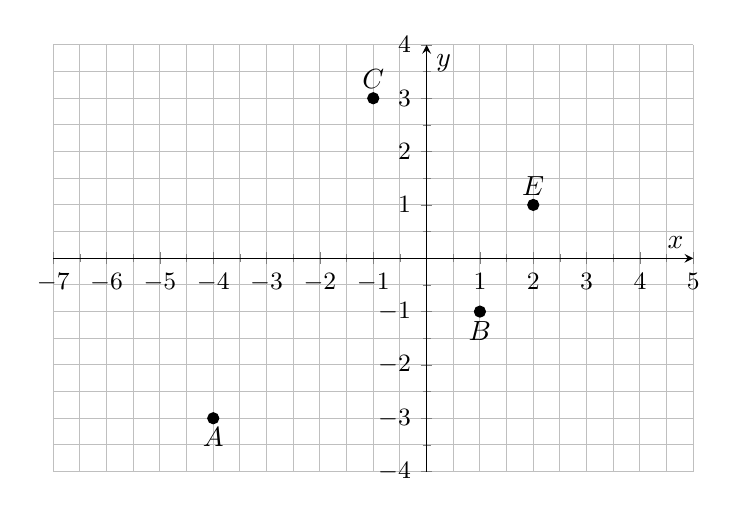
\begin{tikzpicture}\begin{axis}[coursaxe,axis equal image,xmin=-7,xmax=5,ymin=-4,ymax=4,width=12cm,height=7cm,xtick={-7,...,5},ytick={-4,...,4}]
\addplot[only marks]coordinates{(-4,-3)(1,-1)(-1,3)(2,1)};
\node[below]at(axis cs:-4,-3){$A$};\node[below]at(axis cs:1,-1){$B$};\node[above]at(axis cs:-1,3){$C$};\node[above]at(axis cs:2,1){$E$};
\ifprof\addplot[thick]coordinates{(-4,-3)(1,-1)(-1,3)(-6,1)(-4,-3)};\addplot[dashed,domain=-6:5]{.4*x-1.4};\addplot[dashed,domain=-2:5]{-2*x/3+7/3};\addplot[only marks]coordinates{(3.5,0)(0,-.333333)};\node[above]at(axis cs:-6,1){$D$};\node[above]at(axis cs:3.5,0){$K$};\node[below right]at(axis cs:0,-.33333){$F$};\fi
\end{axis}\end{tikzpicture}\end{center}
\reponse[4]{1. $D=A+C-B=(-6;1)$. 2. Milieu de $[AC]$ et de $[BD]$ : $I(-5/2;0)$. 3. $(AB):2x-5y-7=0$ ; $(CE):2x+3y-7=0$. Soustraire donne $8y=0$, puis $x=7/2$, donc $K(7/2;0)$. 4. $\vect{AE}=(6;4)$, donc $F=A+(4;8/3)=(0;-1/3)$. $\vect{DF}=(6;-4/3)$, $\vect{DB}=(7;-2)$ ; déterminant $-12+28/3=-8/3\ne0$. Les trois points ne sont pas alignés.}

\fiche{Comparer une méthode vectorielle et une méthode repérée}
\ex{Dans un triangle non aplati $ABC$, $I$ est le milieu de $[AB]$ et $J$ le milieu de $[AC]$.
\begin{enumerate}\item Démontrer vectoriellement que $(IJ)\parallel(BC)$.\item Vérifier avec $A(0;0)$, $B(6;0)$, $C(2;4)$.\item Pour ces coordonnées, déterminer les équations de $(IJ)$ et $(BC)$, puis le rapport $IJ/BC$.\end{enumerate}}
\reponse[7]{1. $\vect{IJ}=\vect{IA}+\vect{AJ}=\frac12(\vect{BA}+\vect{AC})=\frac12\vect{BC}$. Les vecteurs sont non nuls et colinéaires.\\2. $I(3;0)$, $J(1;2)$ ; $\vect{IJ}=(-2;2)$ et $\vect{BC}=(-4;4)$.\\3. $(IJ):x+y-3=0$ ; $(BC):x+y-6=0$. Leurs directeurs sont colinéaires. $IJ=\sqrt8$, $BC=\sqrt{32}$, donc $IJ/BC=1/2$. La preuve vectorielle est générale ; la vérification numérique ne démontre que ce cas particulier.}
\ex{Une figure semble montrer deux droites parallèles. Quelle différence y a-t-il entre cette observation et une preuve ?}
\reponse[3.2]{La figure suggère une conjecture et peut être imprécise. Une preuve utilise des données exactes et une propriété, par exemple un déterminant nul de vecteurs directeurs non nuls. Une conclusion doit préciser les objets concernés.}

\fiche{Reconnaître une configuration et justifier}
\ex[Situation créée]{Dans un repère orthonormé, $A(0;0)$, $B(4;2)$, $C(3;4)$ et $D(-1;2)$.
\begin{enumerate}\item Montrer que $ABCD$ est un parallélogramme.\item Calculer les quatre longueurs et déterminer s'il s'agit d'un losange.\item Calculer $AC^2$, $BD^2$ et déterminer s'il s'agit d'un rectangle.\item Déterminer son centre et une équation de chaque diagonale.\end{enumerate}}
\reponse[8]{1. $\vect{AB}=(4;2)=\vect{DC}$ : c'est un parallélogramme. 2. $AB=CD=\sqrt{20}=2\sqrt5$, $BC=DA=\sqrt5$ ; les côtés adjacents ne sont pas égaux, donc pas un losange. 3. $AC^2=3^2+4^2=25$ ; $BD^2=(-5)^2+0^2=25$. Un parallélogramme dont les diagonales ont la même longueur est un rectangle. On peut aussi utiliser $AB^2+BC^2=20+5=25=AC^2$ et la réciproque de Pythagore. 4. Le centre est $I(3/2;2)$. $(AC):4x-3y=0$ ; $(BD):y=2$. Leur intersection retrouve $I$.}
\prof{Comparaison de démarches : une preuve par Pythagore ou par propriété des diagonales suffit. Ne pas imposer le produit scalaire, qui n'est pas nécessaire ici. Pour l'oral, répartir les méthodes entre groupes, puis demander une justification commune.}

\sequence{Problèmes de synthèse, raisonnement et automatismes}{Synthèse et raisonnement}{30 mars--9 avril 2027}
\section{Implication, réciproque et contre-exemple}
\begin{cours}[Outils à utiliser en situation]
« Si $P$, alors $Q$ » est une implication $P\Rightarrow Q$. Sa réciproque est $Q\Rightarrow P$ ; elle n'est pas automatiquement vraie. Une équivalence $P\iff Q$ exige les deux implications.
Un contre-exemple suffit à réfuter une assertion universelle ; quelques exemples ne suffisent pas à la prouver. La contraposée $\text{non }Q\Rightarrow\text{non }P$ est équivalente à $P\Rightarrow Q$.
\end{cours}
\ex{Pour un entier $n$ : « Si $n$ est multiple de $4$, alors $n$ est pair. » Démontrer l'implication, écrire sa réciproque et sa contraposée, puis dire lesquelles sont vraies.}
\reponse[5]{Si $n=4k$, alors $n=2(2k)$ est pair. Réciproque : « Si $n$ est pair, alors $n$ est multiple de $4$ » ; elle est fausse avec $n=2$. Contraposée : « Si $n$ est impair, alors $n$ n'est pas multiple de $4$ » ; elle est vraie et équivalente à l'implication initiale.}
\ex{Pour $x\in\R$, étudier « $x=3\Rightarrow x^2=9$ » et sa réciproque. Donner une équivalence correcte.}
\reponse[3.2]{L'implication est vraie. La réciproque est fausse avec $x=-3$. L'équivalence correcte est $x^2=9\iff x=3\text{ ou }x=-3$. Avec l'hypothèse supplémentaire $x\geq0$, on peut écrire $x^2=9\iff x=3$.}
\prof{Ces notions sont explicitées à partir des problèmes ; elles ne constituent pas un chapitre autonome de logique formelle à mémoriser sans contexte.}

\fiche{Négation, disjonction de cas et preuve}
\ex{Nier correctement : « $x>2$ » ; « $x\in[1;4]$ » ; « Tous les élèves font du sport » ; « $A$ et $B$ sont réalisés ».}
\reponse[4]{« $x\leq2$ » ; « $x<1$ ou $x>4$ » ; « Au moins un élève ne fait pas de sport » ; « $A$ n'est pas réalisé ou $B$ n'est pas réalisé ». Le « ou » est inclusif.}
\ex{Montrer par disjonction de cas que $n(n+1)$ est pair pour tout entier $n$. Montrer ensuite que $n^2+n+1$ est impair.}
\reponse[4]{Si $n$ est pair, $n(n+1)$ a un facteur pair. Si $n$ est impair, $n+1$ est pair ; le produit est encore pair. Les deux cas couvrent tous les entiers. Comme $n^2+n+1=n(n+1)+1$, c'est un entier impair.}
\ex{Un élève écrit « $n^2$ pair implique $n$ pair, parce que je l'ai vérifié pour $n=2,4,6$ ». Remplacer cette justification par une preuve.}
\reponse[3.2]{Si $n$ était impair, le résultat démontré en séquence 1 donnerait $n^2$ impair, contradiction. C'est un raisonnement par contraposée, ou présenté ici par l'absurde. Trois exemples ne traitent pas tous les entiers.}

\fiche{Croiser algèbre, fonctions et pourcentages}
\ex[Situation créée]{Deux tarifs fictifs de location sont proposés pour $x$ heures, avec $x\in[0;8]$ : $A(x)=3000+2000x$ Ar et $B(x)=3500x$ Ar.
\begin{enumerate}\item Calculer les coûts pour $1$ h et $4$ h.\item Trouver l'égalité des tarifs puis les durées où $A$ est moins cher.\item Une remise de $10\,\%$ est accordée sur tout le tarif $A$. Donner le nouveau tarif $A_r$ et le nouveau seuil de comparaison.\end{enumerate}}
\reponse[6]{1. À $1$ h : $5000$ Ar contre $3500$ Ar. À $4$ h : $11000$ Ar contre $14000$ Ar. 2. $3000+2000x=3500x\iff x=2$. $A<B$ pour $x>2$, donc sur $]2;8]$. 3. $A_r(x)=0{,}9(3000+2000x)=2700+1800x$. L'égalité avec $B$ donne $1700x=2700$, soit $x=27/17\approx1{,}59$ h. $A_r<B$ sur $]27/17;8]$. La remise s'applique aussi au forfait fixe.}
\begin{lstlisting}
def tarif_moins_cher(x):
    a = 3000 + 2000*x
    b = 3500*x
    if a < b:
        return "A"
    elif b < a:
        return "B"
    else:
        return "egalite"
\end{lstlisting}
\ex{Prévoir les résultats pour $x=1,2,4$. Modifier la ligne qui calcule $a$ pour prendre en compte la remise.}
\reponse[2.4]{Résultats : \texttt{"B"}, \texttt{"egalite"}, \texttt{"A"}. Remplacer par \texttt{a = 0.9*(3000 + 2000*x)}. Le domaine $[0;8]$ est supposé respecté lors des appels.}

\sequence{Probabilités : conditionnement et arbres pondérés}{Probabilités}{26 avril--24 mai 2027}
\section{Univers, issues et événements}
\begin{cours}[Vocabulaire]
Une expérience aléatoire possède plusieurs résultats possibles sans que l'on sache à l'avance lequel sera obtenu. Une issue est un résultat possible ; l'univers $\Omega$ est leur ensemble. Un événement est une partie de $\Omega$ ; un événement élémentaire contient une seule issue.
L'événement impossible est $\varnothing$ ; l'événement certain est $\Omega$.
\end{cours}
\begin{cours}[Opérations sur les événements]
$\overline A$ est l'événement contraire de $A$. $A\cap B$ signifie « $A$ et $B$ » ; $A\cup B$, « $A$ ou $B$ », éventuellement les deux. Deux événements sont incompatibles si $A\cap B=\varnothing$ ; sinon, ils sont compatibles.
\end{cours}
\ex{On lance un dé à six faces. Écrire $\Omega$, $A$ : « obtenir un nombre pair », $B$ : « obtenir $4$ », puis $\overline A$, $A\cap B$ et $A\cup B$. $A,B$ sont-ils compatibles ?}
\reponse[4]{$\Omega=\{1;2;3;4;5;6\}$, $A=\{2;4;6\}$, $B=\{4\}$, $\overline A=\{1;3;5\}$, $A\cap B=\{4\}$, $A\cup B=A$. Les événements sont compatibles car ils partagent l'issue $4$.}
\ex{Avec $A=\{a;b;c;d;e\}$ et $B=\{b;e;f;g;h\}$, donner l'intersection et la réunion. Peut-on déterminer $\overline A$ sans préciser l'univers ?}
\reponse[3.2]{$A\cap B=\{b;e\}$ et $A\cup B=\{a;b;c;d;e;f;g;h\}$. Le complémentaire dépend de l'univers ; on ne peut pas le déterminer sans cette information.}

\fiche{Modèle probabiliste et équiprobabilité}
\begin{cours}[Probabilité dans un univers fini]
À chaque issue, un modèle associe une probabilité positive ou nulle ; la somme vaut $1$. La probabilité d'un événement est la somme des probabilités de ses issues. On a
\[P(\Omega)=1,\quad P(\varnothing)=0,\quad P(\overline A)=1-P(A).\]
En équiprobabilité, toutes les issues ont même probabilité et
\[P(A)=\frac{\Card(A)}{\Card(\Omega)}.\]
L'équiprobabilité est une hypothèse du modèle, pas une conséquence de la seule liste des issues.
\end{cours}
\ex{On suppose le dé équilibré. Pour $A=$ « pair » et $C=$ « supérieur ou égal à $5$ », calculer $P(A)$, $P(C)$, $P(A\cap C)$ et $P(A\cup C)$.}
\reponse[4]{$P(A)=3/6=1/2$, $P(C)=2/6=1/3$, $A\cap C=\{6\}$ donc $P(A\cap C)=1/6$. $A\cup C=\{2;4;5;6\}$, donc $P(A\cup C)=4/6=2/3$. L'issue $6$ ne doit pas être comptée deux fois.}
\ex{Une punaise peut tomber pointe vers le haut ou vers le bas. Peut-on en déduire que chaque issue a probabilité $1/2$ ? Comment proposer un modèle ?}
\reponse[4]{Non : deux issues ne suffisent pas à imposer l'équiprobabilité. On peut répéter les lancers dans des conditions comparables et utiliser les fréquences observées pour proposer un modèle, en gardant à l'esprit les fluctuations et les caractéristiques de l'objet.}
\prof{Réactiver le lien entre fréquence observée et probabilité postulée. Un résultat expérimental ne démontre pas une équiprobabilité exacte.}

\fiche{Probabilité conditionnelle à partir d'un tableau}
\begin{cours}[Définition]
Pour $P(A)>0$, la probabilité de $B$ sachant $A$ est
\[P_A(B)=\frac{P(A\cap B)}{P(A)},\qquad P(A\cap B)=P(A)P_A(B).\]
Dans un tirage équiprobable au sein d'une population finie :
\[P_A(B)=\frac{\Card(A\cap B)}{\Card(A)}.\]
On note aussi $P(B\mid A)$. $P_A(B)$ et $P_B(A)$ ne sont généralement pas égales.
\end{cours}
\ex{On tire uniformément un élève de la classe de $32$ élèves étudiée précédemment. $G$ : « garçon », $N$ : « suit NSI ».}
\begin{center}\renewcommand{\arraystretch}{1.5}\begin{tabular}{c|rr|r}
&$G$&$\overline G$&Total\\\hline
$N$&12&9&21\\$\overline N$&6&5&11\\\hline Total&18&14&32
\end{tabular}\end{center}
Calculer $P(G)$, $P(N)$, $P(G\cap N)$, $P_N(G)$ et $P_G(N)$.
\reponse[5]{$P(G)=18/32=9/16$, $P(N)=21/32$, $P(G\cap N)=12/32=3/8$.
$P_N(G)=12/21=4/7$, tandis que $P_G(N)=12/18=2/3$.
Par la formule : $P_N(G)=(12/32)/(21/32)=12/21$. Sachant que l'élève suit NSI, la population de référence est réduite aux $21$ élèves concernés.}
\vigilance{Le conditionnement exige une probabilité non nulle de l'événement connu ; on ne divise pas par zéro.}

\fiche{Arbres pondérés et probabilité d'un chemin}
\begin{cours}[Règles]
À chaque nœud, la somme des probabilités des branches sortantes vaut $1$. Une branche du deuxième niveau porte une probabilité conditionnelle. Un chemin représente une intersection d'événements ; sa probabilité est le produit des probabilités inscrites sur ce chemin.
\end{cours}
\begin{center}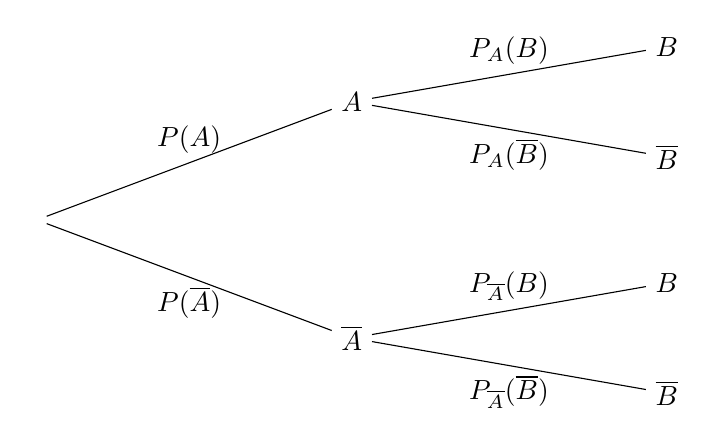
\begin{tikzpicture}[grow=right,level 1/.style={level distance=4cm,sibling distance=3cm},level 2/.style={level distance=4cm,sibling distance=1.4cm},edge from parent/.style={draw},every node/.style={font=\normalsize}]
\node{} child{node{$\overline A$} child{node{$\overline B$} edge from parent node[below]{$P_{\overline A}(\overline B)$}} child{node{$B$} edge from parent node[above]{$P_{\overline A}(B)$}} edge from parent node[below]{$P(\overline A)$}} child{node{$A$} child{node{$\overline B$} edge from parent node[below]{$P_A(\overline B)$}} child{node{$B$} edge from parent node[above]{$P_A(B)$}} edge from parent node[above]{$P(A)$}};
\end{tikzpicture}\end{center}
\ex{On sait $P(A)=0{,}6$, $P_A(B)=0{,}7$ et $P_{\overline A}(\overline B)=0{,}9$. Compléter les autres branches et calculer les probabilités des quatre chemins.}
\reponse[5]{$P(\overline A)=0{,}4$, $P_A(\overline B)=0{,}3$, $P_{\overline A}(B)=0{,}1$.
\[P(A\cap B)=0{,}6\times0{,}7=0{,}42,\quad P(A\cap\overline B)=0{,}18,\]
\[P(\overline A\cap B)=0{,}04,\qquad P(\overline A\cap\overline B)=0{,}36.\]
La somme des quatre probabilités vaut $1$, ce qui contrôle la cohérence du modèle.}
\ex{Justifier la multiplication sur le chemin $A$ puis $B$ à partir de la définition de $P_A(B)$.}
\reponse[2.4]{Comme $P_A(B)=P(A\cap B)/P(A)$ et $P(A)>0$, multiplier par $P(A)$ donne $P(A)P_A(B)=P(A\cap B)$.}

\fiche{Passer d'un tableau à un arbre}
\ex{Pour la classe de $32$ élèves, construire un arbre commençant par NSI / pas de NSI, puis garçon / fille. Construire ensuite l'arbre dans l'ordre inverse. Vérifier, dans les deux arbres, la probabilité de choisir une fille suivant NSI.}
\reponse[7]{Premier arbre : branches initiales $P(N)=21/32$, $P(\overline N)=11/32$. Après $N$ : $P_N(G)=12/21=4/7$, $P_N(\overline G)=9/21=3/7$. Après $\overline N$ : $6/11$ et $5/11$.
Second arbre : branches initiales $P(G)=18/32=9/16$, $P(\overline G)=14/32=7/16$. Après $G$ : $P_G(N)=12/18=2/3$, puis $1/3$. Après $\overline G$ : $P_{\overline G}(N)=9/14$, puis $5/14$.
Le chemin recherché vaut $(21/32)(9/21)=9/32$ dans le premier arbre et $(14/32)(9/14)=9/32$ dans le second. Le changement d'ordre conserve les probabilités des intersections mais change les probabilités des branches.}
\ex{Une urne contient $3$ boules rouges et $2$ bleues. On tire successivement deux boules \textbf{sans remise}. Construire l'arbre des couleurs et calculer la probabilité de tirer deux rouges.}
\reponse[5]{Premier niveau : $R$ avec $3/5$, $B$ avec $2/5$. Après $R$, il reste $2$ rouges et $2$ bleues : branches $1/2,1/2$. Après $B$, il reste $3$ rouges et $1$ bleue : branches $3/4,1/4$. Donc $P(R_1\cap R_2)=(3/5)(1/2)=3/10$. Utiliser $3/5$ sur la seconde branche rouge ignorerait l'absence de remise.}

\fiche{Inversion des conditionnements et faux positifs}
\ex[Contrôle fictif de composants]{Un lot contient $10000$ composants, dont $100$ défectueux. Un test est positif pour $99$ des composants défectueux et pour $495$ des composants non défectueux. On choisit uniformément un composant. $D$ : « défectueux » ; $T$ : « test positif ».
\begin{enumerate}\item Compléter le tableau croisé test / état réel.\item Calculer $P_D(T)$ et $P_T(D)$.\item Donner le nombre de faux positifs et de faux négatifs.\item Calculer la sensibilité $P_D(T)$ et la spécificité $P_{\overline D}(\overline T)$.\end{enumerate}}
\reponse[7]{
\begin{center}\renewcommand{\arraystretch}{1.5}\begin{tabular}{c|rr|r}&$D$&$\overline D$&Total\\\hline $T$&99&495&594\\$\overline T$&1&9405&9406\\\hline Total&100&9900&10000\end{tabular}\end{center}
$P_D(T)=99/100=99\,\%$. En revanche $P_T(D)=99/594=1/6\approx16{,}67\,\%$. Un test positif n'implique donc pas ici une probabilité de défaut de $99\,\%$.
Les $495$ faux positifs sont les composants sains testés positifs ; le faux négatif est le composant défectueux testé négatif. La sensibilité vaut $99\,\%$ ; la spécificité $9405/9900=95\,\%$.
La faible proportion initiale de composants défectueux explique pourquoi les faux positifs sont plus nombreux que les vrais positifs malgré la bonne sensibilité.}
\begin{cours}[Lire le résultat d'un test]
« Positif parmi les défectueux » et « défectueux parmi les positifs » correspondent à deux conditionnements différents. Toujours nommer le groupe de référence avant le calcul.
\end{cours}
\prof{Les nombres sont fictifs. Le tableau permet d'étudier l'inversion sans exiger une formule générale des probabilités totales : celle-ci n'est pas un attendu du programme de seconde 2026.}

\fiche{Simulation et loi des grands nombres}
\begin{cours}[Version vulgarisée]
Lorsqu'on répète un grand nombre de fois une expérience dans le même modèle avec des répétitions indépendantes, la fréquence observée d'un événement est, sauf exception, proche de sa probabilité. Elle fluctue : elle ne s'en rapproche pas nécessairement à chaque nouvelle expérience.
\end{cours}
\begin{lstlisting}
from random import Random

def frequences_six(n, graine=1):
    # n entier >= 1 ; modele de lancers independants
    rng = Random(graine)
    succes = 0
    frequences = []
    for k in range(1, n+1):
        if rng.randint(1, 6) == 6:
            succes = succes+1
        frequences.append(succes/k)
    return frequences
\end{lstlisting}
\ex{Tracer les fréquences pour $n=1000$, avec plusieurs graines. Comparer à $1/6$. Pourquoi fixer la graine ? Peut-on exiger que la fréquence finale soit exactement $1/6$ ?}
\reponse[4]{Les tracés dépendent de la graine et fluctuent autour de $1/6$. Fixer la graine rend la simulation reproductible. Avec $1000$ lancers, une fréquence finale exactement $1/6$ est même impossible, car $1000/6$ n'est pas entier. Une fréquence proche est cohérente avec le modèle, mais n'en constitue pas une démonstration.}
\ex{Modifier le programme pour suivre la fréquence de l'événement « résultat pair ». Quelle probabilité de référence utiliser ?}
\reponse[3.2]{Remplacer le test par \texttt{rng.randint(1, 6) \% 2 == 0}. La probabilité de référence est $3/6=1/2$. Chaque expérience doit effectuer un seul tirage ; ne pas appeler plusieurs fois le générateur pour tester un même résultat.}

\sequence{Consolidation et transition vers la Première}{Bilan annuel}{25 mai--11 juin 2027}
\section{Bilan de calcul, fonctions et géométrie}
\ex[Bilan annuel -- partie A]{\begin{enumerate}
\item Rendre $168/252$ irréductible ; calculer $2^{-3}+1/4$.
\item Factoriser $x^2-6x+9$, puis résoudre $(x-3)^2=4$.
\item Résoudre $\dfrac{x-2}{x+1}\geq0$.
\item Pour $f(x)=4-(x-1)^2$ sur $[-2;3]$, donner le maximum et les abscisses où $f(x)=0$.
\item Avec $A(0;1)$, $B(4;3)$, $C(6;4)$, démontrer l'alignement et donner une équation de la droite.
\end{enumerate}}
\reponse[9]{1. $168/252=2/3$, et $2^{-3}+1/4=1/8+2/8=3/8$. 2. $(x-3)^2$ ; $x-3=\pm2$, donc $S=\{1;5\}$. 3. Interdit $-1$, zéro $2$ ; signes $+,-,+$, donc $S=]-\infty;-1[\cup[2;+\infty[$. 4. Le carré est positif ou nul, donc $f(x)\leq4$, égalité en $x=1$. Les zéros sont $x=-1,3$, tous deux dans le domaine. 5. $\vect{AB}=(4;2)$, $\vect{AC}=(6;3)=\frac32\vect{AB}$. Une équation est $x-2y+2=0$.}
\prof{Barème indicatif : 10 points, 2 par question. Pour la question 3, réserver un point au domaine et aux bornes. Pour la question 5, demander la conclusion après le calcul.}

\fiche{Bilan de données, probabilités et modélisation}
\ex[Bilan annuel -- partie B]{\begin{enumerate}
\item Calculer moyenne et médiane de $2;4;4;6;9$. Déterminer $Q_1,Q_3$.
\item Un prix baisse de $15\,\%$, puis augmente de $20\,\%$. Donner le taux global et le taux permettant ensuite de revenir au prix initial.
\item Dans une population fictive de $100$ personnes, $40$ font du sport ($S$), $30$ viennent à vélo ($V$), $18$ font les deux. Construire le tableau croisé et calculer $P_S(V)$, $P_V(S)$ pour un tirage équiprobable.
\item Pour un rectangle de périmètre $24$ m, exprimer l'aire en fonction d'une dimension $x$ et démontrer son maximum.
\end{enumerate}}
\reponse[9]{1. Moyenne $25/5=5$, médiane $4$. Rangs des quartiles $2$ et $4$, donc $Q_1=4$, $Q_3=6$.\\2. Coefficient global $0{,}85\times1{,}20=1{,}02$ : hausse de $2\,\%$. Taux réciproque $1/1{,}02-1=-1/51\approx-1{,}96\,\%$.\\3. Tableau : $S\cap V=18$, $S\cap\overline V=22$, $\overline S\cap V=12$, $\overline S\cap\overline V=48$. $P_S(V)=18/40=45\,\%$, $P_V(S)=18/30=60\,\%$.\\4. $A(x)=x(12-x)=36-(x-6)^2$ sur $]0;12[$. Le maximum vaut $36$ m$^2$, atteint pour le carré de côté $6$ m.}
\prof{Barème indicatif : 10 points, respectivement 2, 2, 3, 3. Le bilan des parties A et B peut être proposé en une heure, puis repris avec les supports de cours.}

\fiche{Choisir une stratégie et préparer la suite}
\ex[Un programme à expliquer]{Pour une fonction donnée $f$, expliquer le programme suivant. Que renvoie-t-il avec $f(x)=x^2$ ?}
\begin{lstlisting}
def tableau(f):
    valeurs = []
    for x in range(-3, 4):
        valeurs.append((x, f(x)))
    return valeurs
\end{lstlisting}
\reponse[3.2]{Il renvoie une liste de couples abscisse--image pour les entiers de $-3$ à $3$ inclus : $(-3,9),(-2,4),(-1,1),(0,0),(1,1),(2,4),(3,9)$. La borne $4$ de \texttt{range} est exclue. Le tableau ne décrit pas les images de tous les réels entre $-3$ et $3$.}
\begin{cours}[Six compétences à mobiliser]
\textbf{Chercher} : essayer, organiser des pistes. \textbf{Modéliser} : choisir variables, domaine et hypothèses. \textbf{Représenter} : passer du texte au tableau, à la figure ou au graphique. \textbf{Raisonner} : justifier et distinguer conjecture et preuve. \textbf{Calculer} : choisir une forme et contrôler les opérations. \textbf{Communiquer} : expliquer clairement avec des notations et unités adaptées.
\end{cours}
\ex[Portfolio de fin d'année]{Choisir un travail réussi et un travail corrigé. Pour chacun, identifier les compétences mobilisées, expliquer une méthode et formuler un objectif personnel pour l'année suivante. Refaire ensuite un exercice correspondant à cet objectif sans regarder la correction.}
\reponse[4]{Il n'y a pas de réponse numérique unique. Une production satisfaisante identifie précisément le problème, la méthode choisie, une justification et un contrôle. L'objectif doit être observable, par exemple : « préciser les valeurs interdites avant de résoudre une équation quotient », plutôt que « devenir meilleur en calcul ».}
\prof{Pour présenter les parcours de Première, s'appuyer sur les enseignements réellement proposés dans l'établissement et sur leurs programmes en vigueur. Le livret ne fixe pas de seuil de note automatique d'orientation.}

\ifprof
\clearpage\renewcommand{\titreseq}{Annexes professeur}\addcontentsline{toc}{section}{Annexes professeur : utilisation et correspondance}
\section*{Utiliser la source commune}
\begin{cours}[Une seule source, deux versions]
La ligne \texttt{\string\proffalse} du préambule produit la version élève ; la remplacer par \texttt{\string\proftrue} produit la version professeur. Les énoncés et les contenus de cours sont communs. Les réponses, démonstrations rédigées, figures corrigées et repères pédagogiques apparaissent seulement en mode professeur.
\end{cours}
Tous les graphiques et schémas sont écrits en TikZ/PGFPlots. Aucune image externe ni page du PDF original n'est nécessaire à la compilation. Compiler deux fois avec PDFLaTeX pour actualiser la table des matières et les liens. Les deux PDF peuvent avoir des paginations différentes ; les références stables sont les numéros de séquence et d'exemple.
\begin{methode}[Repères de mise en œuvre]
\begin{itemize}
\item Avant un exemple : faire reformuler les données et la question ; autoriser une représentation préparatoire.
\item Pendant la recherche : fournir une aide ciblée (première étape, schéma, cas simple) et une extension aux élèves qui ont terminé.
\item À la correction : séparer résultat, méthode, justification et vérification. Faire expliquer une erreur fréquente.
\item Pour les automatismes : mélanger des questions récentes et plus anciennes, puis refaire après un délai les questions fragiles.
\item Pour la langue : expliciter « parmi », « au moins », « si », « et », « ou » et le sens des symboles avant le calcul.
\end{itemize}
\end{methode}
\section*{Critères communs pour une production}
\begin{center}\small\renewcommand{\arraystretch}{1.6}\begin{tabularx}{\linewidth}{l X}
Chercher&Une démarche est engagée ; les essais apportent une information.\\
Modéliser&Les variables, le domaine et les hypothèses correspondent à la situation.\\
Représenter&Le tableau, graphique ou schéma est lisible, légendé et cohérent.\\
Raisonner&Les propriétés sont appliquées sous leurs conditions ; la conclusion suit.\\
Calculer&Les opérations sont correctes ; les valeurs exactes sont conservées lorsque nécessaire.\\
Communiquer&La rédaction répond à la question, avec unités et précision appropriées.
\end{tabularx}\end{center}
Pour chaque critère, on peut retenir quatre niveaux : non engagé, partiel, correct avec aide, autonome. Cette grille sert à donner un retour exploitable ; elle ne remplace pas un barème propre à une évaluation.

\clearpage\section*{Correspondance avec le livret d'origine}
\begin{center}\small\renewcommand{\arraystretch}{1.5}\begin{tabularx}{\linewidth}{p{6.3cm} X}
\textbf{Séquences du livret fourni}&\textbf{Destination dans cette adaptation}\\\hline
1. Calcul littéral&8 ; réactivation dans les rituels dès la rentrée.\\
2. Nombres et calculs&1 pour l'arithmétique ; 4 pour les ensembles ; 8 pour puissances, fractions et racines.\\
3. Intervalles et valeur absolue&4 ; réinvestissement de la fonction valeur absolue en 6 et 10.\\
4. Équations et inéquations&8 ; équations simples réactivées en 3 et 6.\\
5. Proportion et évolution&9.\\
6. Les vecteurs&2.\\
7. Fonctions et représentation graphique&6 pour représentations et lectures ; 10 pour variations et extrémums.\\
8. Notions de probabilité&14 ; vocabulaire ensembliste introduit en 1.\\
9. Notions de colinéarité&2 ; grande synthèse déplacée en 12.\\
10. Tableau de signes et inéquations&8.\\
11. Statistique&7, avec compléments sur les graphiques et la médiane estimée.\\
12. Droites et systèmes&3.\\
13. Fonctions de référence (4 parties)&3 pour la droite affine ; 6 pour les références et résolutions ; 10 pour les variations.\\
14. Fréquences et probabilités conditionnelles&11 pour les fréquences ; 14 pour le conditionnement et les arbres.\\\hline
Temps de progression sans équivalent direct&5, 12, 13, 15 : bilans, synthèses et consolidation créés.
\end{tabularx}\end{center}
La maquette est reconstruite dans l'esprit du modèle : A4 portrait, typographie sérif, encadrés noirs, zones quadrillées, exemples et démonstrations. La recomposition et le changement d'ordre ne constituent pas un fac-similé page à page. La pagination est continue ; le sommaire n'utilise plus des numéros de page redémarrant à chaque ancienne séquence.
Les exemples numériques exploitables du modèle ont été repris. Des figures ambiguës ont été remplacées par des courbes dont l'expression permet une vérification exacte. Les développements sur racine carrée, cube, simulation, données croisées et bilans complètent la progression. Les situations ajoutées à données inventées sont signalées comme fictives ; une collecte de classe est proposée pour travailler aussi sur des données réelles.

\clearpage\section*{Corrections de fond apportées au modèle}
\begin{enumerate}
\item \textbf{Puissances.} Le produit répété vaut pour un exposant entier strictement positif ; les exposants négatifs exigent une base non nulle.
\item \textbf{Fractions.} Un quotient nul doit être défini ; seule une fraction non nulle possède un inverse. Les simplifications ne suppriment pas les restrictions initiales.
\item \textbf{PGCD.} Les deux entiers ne sont pas tous deux nuls dans la définition par le plus grand diviseur ; $\pgcd(0,0)=0$ est une convention séparée.
\item \textbf{Vecteurs.} Le vecteur nul ne dirige aucune droite. La caractérisation $\vec u=k\vec v$ exige $\vec v\ne\vec0$, ou un traitement séparé du cas nul. La multiplication par tout réel est explicitée.
\item \textbf{Équations de droites.} La condition est $(a,b)\ne(0,0)$ ; l'ordre des vecteurs dans le déterminant a été rendu cohérent. $\vect{AM}$ peut être nul lorsque $M=A$ et n'est alors pas un directeur.
\item \textbf{Intervalles.} $0$ est exclu de l'ensemble des réels strictement négatifs. Les infinis ne sont pas des nombres réels.
\item \textbf{Racines.} Les conditions de positivité et $\sqrt{x^2}=|x|$ sont explicites. Une formule fausse en général n'est pas nécessairement une inégalité toujours vraie.
\item \textbf{Fonctions.} Images et antécédents sont distingués ; les domaines des courbes couvrent les valeurs demandées. Les lectures graphiques ne sont pas affichées avec une précision injustifiée. La fonction inverse n'est pas déclarée décroissante sur tout $\R^*$.
\item \textbf{Statistiques.} La médiane utilise « au moins la moitié ». L'ajout d'une valeur ne fait pas diminuer l'étendue. Les recalculs utilisent la somme exacte $1217$. Variance et écart type ne sont pas des fonctions linéaires des données : leurs transformations correctes sont précisées.
\item \textbf{Classes.} Une série continue n'est pas définie par son seul regroupement. Moyenne à partir des centres et médiane interpolée sont des estimations sous hypothèses, distinctes des valeurs exactes.
\item \textbf{Interprétation.} Une multiplication des notes n'est pas assimilée à une augmentation de difficulté. Proportion, taux et points de pourcentage sont distingués.
\item \textbf{Probabilités.} Les populations de référence et les hypothèses de modèle sont nommées. Inversion des conditionnements, faux positifs, faux négatifs et fluctuations sont travaillés. Aucune formule générale des probabilités totales n'est exigée.
\item \textbf{Optimisation.} Le balayage donne un maximum sur une grille ; une preuve séparée établit le maximum sur l'intervalle. Une dichotomie de recherche de zéro n'est pas présentée comme une méthode générale d'optimisation.
\end{enumerate}

\clearpage\section*{Références et contrôle de couverture}
\textbf{Document de progression retenu :} \emph{Programmation annuelle Seconde 2026--2027 rectifiée finale}, DOCX fourni. Dates et quinze étapes reprises ; les dates indiquent des plages, pas des séances sur les jours fériés.
\par\textbf{Document de départ :} \emph{Livret\_2nde\_\_\_Eleve.pdf}, 91 pages, fourni pour cette adaptation. La source LaTeX d'origine n'étant pas jointe, la présente source est une reconstruction.
\par\textbf{Programme officiel :} arrêté du 26 février 2026, BO n\textsuperscript{o} 14 du 2 avril 2026, NOR MENE2602914A, applicable à la rentrée 2026--2027 :
\par\url{https://www.education.gouv.fr/bo/2026/Hebdo14/MENE2602914A}
\par\textbf{Ressources fournies :} programme de seconde ; ressources « Automatismes 2de » et « Raisonnement et démonstration 2de ». Le livret ne prétend pas reproduire intégralement ces ressources.
\begin{center}\small\renewcommand{\arraystretch}{1.5}\begin{tabularx}{\linewidth}{p{8cm} X}
\textbf{Domaine / capacité}&\textbf{Séquences}\\\hline
Entiers, multiples, parité, fractions irréductibles&1, 5, 8, 13\\
Réels, intervalles, distance, encadrements&4, 5, 8\\
Calcul littéral, puissances, racines, équations et signes&8 ; rituels toute l'année\\
Vecteurs, bases, coordonnées, normes, déterminant&2, 12\\
Équations de droites et intersections&3, 12\\
Représentations et six fonctions de référence&6, 10\\
Variations, extrémums, comparaison, optimisation&10, 13, 15\\
Proportions et évolutions&9, 13, 15\\
Statistiques, dispersion, classes, histogramme, cumulées&7\\
Tableaux croisés, fréquences, données réelles&11\\
Conditionnement, arbres, inversion, simulation&14\\
Logique, preuves, Python, six compétences&Répartis dans les séquences et bilans
\end{tabularx}\end{center}
\textbf{Contrôle mathématique :} les calculs numériques, expressions algébriques, ensembles solutions, données des tableaux, coordonnées et programmes ont fait l'objet d'une relecture et de vérifications calculatoires. Pour les collectes et productions ouvertes, la correction fournit des critères de validité plutôt qu'un résultat inventé. Les estimations et modèles restent explicitement signalés.
\fi

\end{document}
